\documentclass{article}
\usepackage[english]{babel}
\usepackage{amsmath,amssymb,graphicx,hyperref,xcolor,alltt}

%%%%%%%%%% Start TeXmacs macros
\newcommand{\nobracket}{}
\newcommand{\tmaffiliation}[1]{\\ #1}
\newcommand{\tmcolor}[2]{{\color{#1}{#2}}}
\newcommand{\tmem}[1]{{\em #1\/}}
\newcommand{\tmop}[1]{\ensuremath{\operatorname{#1}}}
\newcommand{\tmstrong}[1]{\textbf{#1}}
\newcommand{\codestar}[1]{\textbf{#1}}
\newcommand{\tmtextbf}[1]{\text{{\bfseries{#1}}}}
\newcommand{\tmtextit}[1]{\text{{\itshape{#1}}}}
\newenvironment{tmcode}[1][]{\begin{alltt} }{\end{alltt}}
%%%%%%%%%% End TeXmacs macros

\begin{document}

\

\title{Fourier analysis}

\author{
  Youjun Hu
  \tmaffiliation{Institute of Plasma Physics, Chinese Academy of Sciences\\
  Email: yjhu@ipp.cas.cn}
}

\maketitle

\begin{abstract}
  These notes review the basic theory of Fourier expansion that are necessary
  for one to use Fourier expansion in numerical codes.
\end{abstract}

\section{Introduction}

This note discusses the Fourier expansion and Discrete Fourier Transform
(DFT), giving step by step derivation of the definition of DFT and its
variations such as the discrete sine transform. I also discuss how to relate
this to the output of some computer libraries (e.g. FFTW).

The Fast Fourier Transform algorithm (FFT) makes the DFT fast enough to solve
many real-life problems, which makes FFT be among the top ten algorithms that
have changed the world. The FFT algorithm remained mysterious to me for many
years until I read Cooley and Tukey's original paper, which turns out to be a
very concise paper and very easy to follow (details are discussed in Append.
\ref{23-3-23-p1}).

\section{Fourier series}

\subsection{Fourier series in terms of trigonometric functions}

If $h (x)$ is a function of period $2 L$, then it can be proved that $h (x)$
can be expressed as the following series
\begin{equation}
  \label{2-25-1} h (x) = \sum_{n = 0}^{\infty} a_n \cos \left( \frac{n \pi}{L}
  x \right) + \sum_{n = 1}^{\infty} b_n \sin \left( \frac{n \pi}{L} x \right),
\end{equation}
which is called Fourier series. [It is not trivial to prove the above
statement (what is needed in the proof is to prove that the set of functions
$\cos (n \pi x / L)$ and $\sin (n \pi x / L)$ with $n = 0, 1, \ldots \infty$
is a ``complete set''{\cite{snieder1994}}). We will not concern us here with
this proof and simply start working with the Fourier series in Eq.
(\ref{2-25-1}).] At this point it is not clear yet what the coefficients $a_n$
and $b_n$ are. These can be obtained by taking product of Eq. (\ref{2-25-1})
with $\cos (j \pi x / L)$ and $\sin (j \pi x / L)$, respectively, and then
integrating form $- L$ to $L$, which gives
\begin{equation}
  a_0 = \frac{1}{2 L} \int_{- L}^L h (x) d x,
\end{equation}
and, for $j \geqslant 1$,
\begin{equation}
  \label{2-25-p1} a_j = \frac{1}{L} \int_{- L}^L h (x) \cos \left( \frac{j
  \pi}{L} x \right) d x,
\end{equation}

\begin{equation}
  \label{2-25-p1m} b_j = \frac{1}{L} \int_{- L}^L h (x) \sin \left( \frac{j
  \pi}{L} x \right) d x.
\end{equation}
Fourier series are often redefined as
\begin{equation}
  \label{2-25-p3} h (x) = \frac{a_0}{2} + \sum_{n = 1}^{\infty} \left[ a_n
  \cos \left( \frac{n \pi}{L} x \right) + b_n \sin \left( \frac{n \pi}{L} x
  \right) \right],
\end{equation}
in order to enable $a_n$ to be uniformly expressed by Eq. (\ref{2-25-p1}).
Fourier series (\ref{2-25-p3}) can be further written as
\begin{equation}
  \label{23-4-3-1} h (x) = \sum_{n = - \infty}^{\infty} \left[ \frac{a_n}{2}
  \cos \left( \frac{n \pi}{L} x \right) + \frac{b_n}{2} \sin \left( \frac{n
  \pi}{L} x \right) \right],
\end{equation}
where $n$ ranges from $- \infty$ to $\infty$, and there is no special
treatment for the edge case of $n = 0$. In obtaining expression
(\ref{23-4-3-1}) from (\ref{2-25-p3}), use has been made of $a_n \cos (n \pi x
/ L) = a_{- n} \cos (- n \pi x / L)$, $b_n \sin (n \pi x / L) = b_{- n} \sin
(- n \pi x / L)$, and $b_0 = 0$.

If $h (x)$ is a complex-valued function (the independent variable $x$ is still
real number), then the above Fourier expansion can be applied to its real part
and imaginary part, respectively. Combining the results, we can see that Eqs.
(\ref{2-25-p1})-(\ref{2-25-p3}) is still valid. In this case, $a_n$ and $b_n$
are complex numbers.

Note that sine and cosine are essentially the same function: one can be
obtained from the other by shifting, i.e., they differs only in the ``phase''.
For the case that $h (x)$ is real-valued, using trigonometric identities,
expression (\ref{2-25-p3}) can be expressed in terms of only cosine/sine
functions:
\begin{equation}
  h (x) = \frac{a_0}{2} + \sum_{n = 1}^{\infty} A_n \cos \left( \frac{n
  \pi}{L} x - \Phi_n \right),
\end{equation}
where the amplitude $A_n$ is given by
\begin{equation}
  \label{20-12-16-a1} A_n = \sqrt{a_n^2 + b_n^2},
\end{equation}
and the phase $\Phi_n$ is given by
\begin{equation}
  \label{20-12-19-a1} \Phi_n = \tmop{atan} 2 (b_n, a_n),
\end{equation}
where $\tmop{atan} 2 (y, x)$ is a Fortran function computing the poloidal
angle of Cartesian point $(x, y)$, which gives an angle in the correct
quadrant.

\subsection{Fourier series in terms of basis functions $e^{i n \pi x / L}$}

Fourier series are often expressed in terms of the complex-valued basis
functions $e^{i n \pi x / L}$. Next, we derive this version of the Fourier
series, which is the most popular version we see in textbooks and papers (we
will see the reason why this version is popular).

Using Euler's formula (this is a bridge between representations using real
numbers and complex numbers)
\begin{equation}
  \cos \left( \frac{n \pi}{L} x \right) = \frac{e^{i n \pi x / L} + e^{- i n
  \pi x / L}}{2}
\end{equation}
and
\begin{equation}
  \sin \left( \frac{n \pi}{L} x \right) = \frac{e^{i n \pi x / L} - e^{- i n
  \pi x / L}}{2 i}
\end{equation}
in Eq. (\ref{2-25-p3}), we obtain
\begin{equation}
  h (x) = \frac{a_0}{2} + \sum_{n = 1}^{\infty} a_n \frac{e^{i n \pi x / L} +
  e^{- i n \pi x / L}}{2} + \sum_{n = 1}^{\infty} b_n \frac{e^{i n \pi x / L}
  - e^{- i n \pi x / L}}{2 i},
\end{equation}
which can be organized as
\begin{equation}
  \label{10-24-e1} h (x) = \frac{a_0}{2} + \sum_{n = 1}^{\infty} \left[ \left(
  \frac{a_n - i b_n}{2} \right) e^{i n \pi x / L} + \left( \frac{a_n + i
  b_n}{2} \right) e^{- i n \pi x / L} \right] .
\end{equation}
And this form motivates us to define
\begin{equation}
  \label{2-25-p4} c_n = \frac{a_n - i b_n}{2}, c_{- n} = \frac{a_n + i
  b_n}{2},
\end{equation}
where $n = 0, 1, 2, \ldots$ (note $b_0 = 0$), then Eq. (\ref{10-24-e1}) is
written
\begin{equation}
  \label{2-25-p6} h (x) = \sum_{n = - \infty}^{\infty} c_n e^{i n \pi x / L} .
\end{equation}
Furthermore, the expressions of $a_n$ and $b_n$ given by Eq. (\ref{2-25-p1})
and (\ref{2-25-p1m}) indicate that $c_n$ and $c_{- n}$ in Eq. (\ref{2-25-p4})
can be uniformly expressed as
\begin{equation}
  \label{2-25-p7} c_n = \frac{1}{2 L} \int_{- L}^L h (x) e^{- i n \pi x / L} d
  x.
\end{equation}
Equation (\ref{2-25-p6}) along with Eq. (\ref{2-25-p7}) is the version of
Fourier series using complex basis functions. In this version, the index $n$
is an integer ranging from negative infinity to positive infinity, which is
unlike Eq. (\ref{2-25-1}), where $n$ is from zero to positive infinity. An
advantage of Eqs. (\ref{2-25-p6}) and (\ref{2-25-p7}) is that no special
treatment is needed for the edge case of $n = 0$.

Using Eq. (\ref{2-25-p7}) in Eqs. (\ref{2-25-p6}), we obtain
\begin{eqnarray}
  h (x) & = & \sum_{n = - \infty}^{\infty} \left( \frac{1}{2 L} \int_{- L}^L h
  (x) e^{- i n \pi x / L} d x \right) e^{i n \pi x / L} . \nonumber\\
  & = & \sum_{n = - \infty}^{\infty} \left( \frac{1}{2 L} \int_{- L}^L h (x)
  \left( \cos \left( \frac{n \pi}{L} x \right) - i \sin \left( \frac{n \pi}{L}
  x \right) \right) d x \right) \left( \cos \left( \frac{n \pi}{L} x \right) +
  i \sin \left( \frac{n \pi}{L} x \right) \right) \nonumber\\
  & = & \sum_{n = - \infty}^{\infty} \left( \frac{1}{2 L} \int_{- L}^L h (x)
  \cos \left( \frac{n \pi}{L} x \right) d x \right) \cos \left( \frac{n
  \pi}{L} x \right) \nonumber\\
  & + & \sum_{n = - \infty}^{\infty} \left( \frac{1}{2 L} \int_{- L}^L h (x)
  \sin \left( \frac{n \pi}{L} x \right) d x \right) \left. \sin \left( \frac{n
  \pi}{L} x \right. \right) \nonumber\\
  & + & \sum_{n = - \infty}^{\infty} \left( \frac{1}{2 L} \int_{- L}^L h (x)
  \left. \cos \left( \frac{n \pi}{L} x \right. \right) d x \right) \left( i
  \sin \left( \frac{n \pi}{L} x \right) \right)  \label{23-4-3-4}\\
  & + & \sum_{n = - \infty}^{\infty} \left( \frac{1}{2 L} \int_{- L}^L h (x)
  \left( - i \sin \left( \frac{n \pi}{L} x \right) \right) d x \right) \left(
  \cos \left( \frac{n \pi}{L} x \right) \right)  \label{23-4-3-5}
\end{eqnarray}
Noting that the $+ n$ terms cancel the $- n$ terms in both line
(\ref{23-4-3-4}) and line (\ref{23-4-3-5}), then $h (x)$ is written as
\begin{eqnarray}
  h (x) & = & \sum_{n = - \infty}^{\infty} \left( \frac{1}{2 L} \int_{- L}^L h
  (x) \cos \left( \frac{n \pi}{L} x \right) d x \right) \cos \left( \frac{n
  \pi}{L} x \right) \nonumber\\
  & + & \sum_{n = - \infty}^{\infty} \left( \frac{1}{2 L} \int_{- L}^L h (x)
  \sin \left( \frac{n \pi}{L} x \right) d x \right) \left. \sin \left( \frac{n
  \pi}{L} x \right. \right)  \label{23-3-27-1}
\end{eqnarray}
Define new expansion coefficients
\begin{equation}
  a_n' = \frac{a_n}{2} = \frac{1}{2 L} \int_{- L}^L h (x) \cos \left( \frac{n
  \pi}{L} x \right) d x
\end{equation}
and
\begin{equation}
  b_n' = \frac{b_n}{2} = \frac{1}{2 L} \int_{- L}^L h (x) \sin \left( \frac{n
  \pi}{L} x \right) d x
\end{equation}
then expression (\ref{23-3-27-1}) is written as
\begin{equation}
  h (x) = \sum_{n = - \infty}^{\infty} a_n' \cos \left( \frac{n \pi}{L} x
  \right) + \sum_{n = - \infty}^{\infty} b_n' \left. \sin \left( \frac{n
  \pi}{L} x \right. \right),
\end{equation}
which recovers expression (\ref{23-4-3-1}). Note that $n \in (- \infty, +
\infty)$ in this version, which differs from Eq. (\ref{2-25-p3}). Also this
expression has no edge case that needs special treatment.

Using Eq. (\ref{2-25-p4}), the coefficients $a_n$ and $b_n$ appearing in Eq.
(\ref{2-25-p3}) can be recovered from $c_n$ by
\begin{equation}
  \label{11-8-e1} a_n = c_n + c_{- n},
\end{equation}
\begin{equation}
  \label{4-18-e1} b_n = i (c_n - c_{- n}) .
\end{equation}
If $h (x)$ is real, then the coefficients $a_n$ and $b_n$ are real. Then
equation (\ref{2-25-p4}) implies that $c_n$ and $c_{- n}$ are complex
conjugates. In this case, expressions (\ref{11-8-e1}) and (\ref{4-18-e1}) are
simplified as
\begin{equation}
  a_n = 2 \tmop{Re} (c_n),
\end{equation}
\begin{equation}
  b_n = - 2 \tmop{Im} (c_n) .
\end{equation}


[In the above, we use the basis functions $e^{i n \pi x / L}$ to expand $h
(x)$. If we choose the basis functions to be $e^{- i n \pi x / L}$, then it is
ready to verify that the Fourier series are written
\begin{equation}
  h (x) = \sum_{n = - \infty}^{\infty} c_n e^{- i n \pi x / L},
\end{equation}
with $c_n$ given by
\begin{equation}
  \label{19-1-10-1} c_n = \frac{1}{2 L} \int_{- L}^L h (x) e^{i n \pi x / L} d
  x.
\end{equation}
In this case, the coefficients $a_n$ and $b_n$ can be recovered from $c_n$ by
\begin{equation}
  \label{18-2-2p1} a_n = c_n + c_{- n}
\end{equation}
\begin{equation}
  \label{18-2-2p2} b_n = - i (c_n - c_{- n})
\end{equation}
In using the Fourier series, we should be aware of which basis functions are
used.]

\subsection{Numerical computation of Fourier expansion coefficient}

For a periodic function $h (t)$ with a period of $T$, Fourier series are
written as
\begin{equation}
  h (t) = \sum_{n = - \infty}^{\infty} c_n \exp \left( \frac{i n 2 \pi t}{T}
  \right),
\end{equation}
with the coefficient $c_n$ given by
\begin{equation}
  \label{19-1-10-1m} c_n = \frac{1}{T} \int_0^T h (t) \exp \left( - \frac{i n
  2 \pi t}{T} \right) d t.
\end{equation}
How to numerically compute the Fourier expansion coefficient? A simple way is
to use the rectangle formula to approximate the integration in Eq.
(\ref{19-1-10-1m}), i.e.,
\begin{equation}
  \label{10-3-e2m} c_n \approx \frac{\Delta}{T} \sum_{j = 0}^{N - 1} h_j \exp
  \left( - \frac{i n 2 \pi j \Delta}{T} \right),
\end{equation}
where $h_j = h (t_j)$ and $t_j = j \Delta$ with $j = 0, 1, 2, \ldots, N - 1$
and $\Delta = T / N$, as is shown in Fig. \ref{16-2-25}.

\begin{figure}[h]
  \resizebox{8cm}{!}{\includegraphics{/home/yj/project_new/fft/fig2c/MyFigure.eps}}
  \caption{\label{16-2-25}Sampling points in one period of the signal, where
  $T = N \Delta$ is the period of the signal.}
\end{figure}

\

Note Eq. (\ref{10-3-e2m}) is an approximation, which will become exact if
$\Delta \rightarrow 0$. In practice, we can sample $h (t)$ only with a nonzero
$\Delta$. Therefore Eq. (\ref{10-3-e2m}) is usually an approximation. Do we
have some rules to choose a suitable $\Delta$ so that Eq. (\ref{10-3-e2m}) can
become a good approximation or even an exact relation? This important question
is answered by the sampling theorem, which sates that a suitable $\Delta$ to
make Eq. (\ref{10-3-e2m}) exact is given by $\Delta \leqslant 1 / (2 f_c)$,
where $f_c = N_c / T$ is the largest frequency contained in $h (t)$ (i.e,
$c_n$ is zero for $| n | \geqslant N_c$).

\section{Discrete Fourier transformation (DFT)}\label{9-29-8}

\subsection{Definition of DFT}

The summation in Eq. (\ref{10-3-e2m}),
\begin{equation}
  \label{2-26-2} H_n \equiv \sum_{j = 0}^{N - 1} h_j \exp \left( - i \frac{2
  \pi}{N} n j \right),
\end{equation}
is called the {\tmstrong{Discrete Fourier transformation (DFT)}}, where $n = -
N / 2, \ldots, 0, \ldots, N / 2$ (we consider only the case that $N$ is an
even number). The Fourier expansion coefficients $c_n$ in Eq. (\ref{10-3-e2m})
is then written as
\begin{equation}
  c_n = \frac{1}{N} H_n .
\end{equation}
The corresponding frequency corresponding to the $c_n$ term is
\begin{equation}
  \label{10-26-1} f_n = f_s \frac{n}{N},
\end{equation}
where $f_s = 1 / \Delta$ is called sampling frequency.

The efficient algorithm of computing the DFT is discussed in Appendix
\ref{18-1-28-a1}.

\subsection{Periodic property of Discrete Fourier transformation}

The DFT of time-domain array $h_j$ with $j = 0, 1, \ldots, N - 1$ is given by
Eq. (\ref{2-26-2}), i.e.,
\begin{equation}
  \label{3-25-e3} H_n = \sum_{j = 0}^{N - 1} W^{n j} h_j
\end{equation}
with $n = - N / 2, \ldots, N / 2$, where $W = \exp (2 \pi i / N)$.

Note that the subscript of $H_n$ is in the range $n = - N / 2, \ldots, N / 2$
while the subscript of $h_j$ is in the range $j = 0, 1, \ldots, N - 1$.
Further note that $H_n$ contains $N + 1$ elements while $h_j$ contains only
$N$ elements. It is ready to find that the array defined in Eq.
(\ref{3-25-e3}) has the following periodic property
\begin{equation}
  \label{3-25-e1} H_{n + N} = H_n .
\end{equation}
Using this general property, we obtain $H_{- N / 2} = H_{N / 2}$, i.e., the
two ending elements of $H_n$, namely $H_{- N / 2}$ and $H_{N / 2}$, are equal
to each other. Thus only one value is needed to be stored. This can be used to
reduce the number of elements of $H_n$ that need to be stored by one. Then
$H_n$ contains only $N$ elements rather than $N + 1$. Furthermore, we prefer
to make the index of $H_n$ and $h_j$ array have the same range, i.e., $[0, N -
1]$. This can be done by storing the negative frequency part (i.e., $n = - N /
2, \ldots, - 1$) of $H_n$ in the locations where the subscripts are
respectively $n = N / 2, \ldots, N - 1$, as is shown in Fig \ref{4-16-1}. A
naive method of implementing this in a code is to first calculate the values
of $H_n$ in the range $n = - N / 2, \ldots, N / 2$, then shift the array to
achieve the desired storage arrangement, as is shown in Fig \ref{4-16-1}. It
turns out that we have a better way to achieve the same goal: using again the
periodic property Eq. (\ref{3-25-e1}), we know that the value of the $H_n$
array elements with negative subscripts, $n = - N / 2, \ldots, - 1$, happens
to be equal to the value of the $H_n$ elements with subscripts $n = N / 2,
\ldots, N - 1$, respectively. Using this, we can simply use Eq.
(\ref{3-25-e3}) to calculate values of $H_n$ in the range $n = 0, 1, N - 1$
and the array obtained is exactly in the desired storage arrangement.

\begin{figure}[h]
  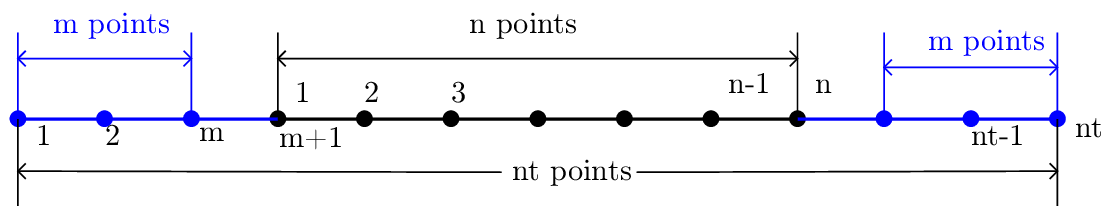
\includegraphics{/home/yj/theory/figures/fft_storage/a-1.eps}
  \caption{\label{4-16-1}The negative frequency parts of the discrete Fourier
  transformation are stored at the locations with the array index $n =
  \frac{N}{2}, \frac{N}{2} + 1, \ldots, N - 1$. Since $H_{- N / 2} = H_{N /
  2}$, the location $j = N / 2$ of the new array can be considered to be
  storing both of them.}
\end{figure}

In practice, we do not use Eq. (\ref{3-25-e3}) directly to calculate $H_n$.
Instead, the famous Fast Fourier Transformation (FFT) algorithm is used to
calculate $H_n$ with $n = 0, 1, \ldots, N - 1$. Remember the storage
arrangement discussed above is important for one to correctly interpret and
use the output of FFT. For example, what frequency does the element $H_j$ with
$j > N / 2$ correspond to? The answer is obvious if we know the storage
arrangement of FFT output: the corresponding frequency of No. $j$th element is
given by
\begin{equation}
  \label{17-10-14-1} f_j = \left\{ \begin{array}{l}
    j \frac{f_s}{N}, \hspace{3em} \tmop{for} \quad 0 \leqslant j \leqslant
    \frac{N}{2}\\
    (j - N) \frac{f_s}{N}, \quad \tmop{for} \quad  \frac{N}{2} < j \leqslant N
    - 1
  \end{array} \right.
\end{equation}
Define $f_1 = f_s / N = 1 / T$, then Eq. (\ref{17-10-14-1}) can be written as
\begin{equation}
  f_j = \left\{ \begin{array}{l}
    j f_1, \hspace{5em} \tmop{for} \quad 0 \leqslant j \leqslant \frac{N}{2}\\
    (j - N) f_1, \qquad \tmop{for} \quad  \frac{N}{2} < j \leqslant N - 1
  \end{array} \right.,
\end{equation}
Here $f_1$ is the spacing in the frequency domain and is called frequency
resolution.

Q: What is the negative frequency counterpart of the element $H_j$ for $j \neq
0$ ?

A: The storage arrangement shown in Fig. \ref{4-16-1} indicates that it is the
element $H_{N - j}$.

\subsection{Frequency resolution and bandwidth}

The frequency interval between neighbor DFT points is $1 / T$, where $T$ is
the time-window in which the signal is sampled. This frequency interval is
called frequency resolution, which is determined only by the length of the
time-window and is independent of the sampling frequency. If the time-window
is fixed, increasing the sampling frequency only increase the bandwidth (the
frequency range of DFT) and the frequency interval between neighbor DFT points
are still $1 / T$, i.e., the frequency resolution is not changed. In summary,
{\tmem{Bandwidth}} is the highest frequency that is captured in the Fourier
transform, equal to half the sampling rate. {\tmem{Frequency Resolution}} is
$1 / T$, which is the spacing between samples in the frequency domain.

\section{Inverse transform}

\subsection{Reconstruct the original function using DFT}

The Fourier series of $h (t)$
\begin{equation}
  h (t) = \sum_{n = - \infty}^{\infty} c_n \exp \left( - i \frac{n 2 \pi t}{T}
  \right),
\end{equation}
can be approximated as
\begin{equation}
  h (t) \approx \sum_{n = - N / 2}^{N / 2} c_n \exp \left( - i \frac{n 2 \pi
  t}{T} \right) .
\end{equation}
Using the relation $c_n = H_n / N$, the above equation is written as
\begin{eqnarray}
  h (t) & = & \frac{1}{N} \sum_{n = - N / 2}^{N / 2} H_n \exp \left( - i
  \frac{n 2 \pi t}{T} \right) \nonumber\\
  & = & \frac{1}{N} \left[ \sum_{n = 0}^{N / 2} H_n \exp \left( - i \frac{n 2
  \pi t}{T} \right) + \sum_{n = - N / 2}^{- 1} H_n \exp \left( - i \frac{n 2
  \pi t}{T} \right) \right] . 
\end{eqnarray}
Using the periodic property of DFT, i.e., $H_n = H_{N + n}$, the above
expression is written as
\begin{eqnarray}
  h (t) & = & \frac{1}{N} \left[ \sum_{n = 0}^{N / 2} H_n \exp \left( - i
  \frac{n 2 \pi t}{T} \right) + \sum_{n = N / 2}^{N - 1} H_n \exp \left( - i
  \frac{(n - N) 2 \pi t}{T} \right) \right] .  \label{11-9-1}
\end{eqnarray}
Equation (\ref{11-9-1}) provides a formula of constructing an approximate
function using the DFT of the discrete samplings of the original function.

\subsection{Evaluate the reconstructed function at discrete points}

Evaluate $h (t)$ given by Eq. (\ref{11-9-1}) at the discrete point $t = j
\Delta$, yielding
\begin{eqnarray}
  h (j \Delta) & = & \frac{1}{N} \left[ \sum_{n = 0}^{N / 2} H_n \exp \left( -
  i \frac{n 2 \pi j}{N} \right) + \sum_{n = N / 2}^{N - 1} H_n \exp \left( - i
  \frac{(n - N) 2 \pi j}{N} \right) \right] . \nonumber\\
  & = & \frac{1}{N} \left[ \sum_{n = 0}^{N / 2} H_n \exp \left( - i \frac{n 2
  \pi j}{N} \right) + \sum_{n = N / 2}^{N - 1} H_n \exp \left( - i \frac{n 2
  \pi j}{N} \right) \right] . \nonumber\\
  & = & \frac{1}{N} \left[ \sum_{n = 0}^{N - 1} H_n \exp \left( - i \frac{n 2
  \pi j}{N} \right) + \tmcolor{blue}{H_{N / 2} \exp (- i \pi j)} \right] . 
\end{eqnarray}
Drop \tmcolor{blue}{the blue term} (which is negligible if $h$ satisfies the
sampling theorem), then $h (j \Delta)$ is written as
\begin{equation}
  \label{11-9-3} h (j \Delta) \approx \frac{1}{N} \sum_{n = 0}^{N - 1} H_n
  \exp \left( - i \frac{n 2 \pi j}{N} \right) .
\end{equation}
The right-hand side of Eq. (\ref{11-9-3}) turns out to be the inverse DFT
discussed in Sec. \ref{11-9-2}.

\subsection{Inverse Discrete Fourier transformation}\label{11-9-2}

The DFT in Eq. (\ref{2-26-2}), i.e.,
\begin{equation}
  \label{21-9-15-p1} H_n \equiv \sum_{j = 0}^{N - 1} h_j \exp \left( i \frac{2
  \pi}{N} n j \right),
\end{equation}
with $j = 0, 1, 2, \ldots, N - 1$ and $n = 0, 1, 2, \ldots, N - 1$ can also be
considered as a set of linear algebraic equations for $h_j$ and can be solved
in terms of $h_j$, which gives
\begin{equation}
  \label{10-7-1} h_j = \frac{1}{N} \sum_{n = 0}^{N - 1} H_n \exp \left( - i
  \frac{2 \pi}{N} n j \right) .
\end{equation}
(The details on how to solve Eq. (\ref{2-26-2}) to obtain the solution
(\ref{10-7-1}) is provided in Sec. \ref{10-7-p5}.) Equation (\ref{10-7-1})
recovers $h_j$ from $H_n$ (i.e., the DFT of $h_j$), and thus is called the
inverse DFT.

The normalization factor multiplying the DFT and inverse DFT (here $1$ and $1
/ N$) and the signs of the exponents are merely conventions, and differ in
some treatments. The only requirements of these conventions are that the DFT
and inverse DFT have opposite-sign exponents and that the product of their
normalization factors be $1 / N$. In most FFT computer libraries, the $1 / N$
factor is omitted. So one must take this factor into account when one wants to
reproduce the original data after a forward and then a backward transform.

\subsection{Proof of the inverse DFT}\label{10-7-p5}

In order to solve the linear algebraic equations (\ref{2-26-2}) for $h_j$,
multiply both sides of each equation by $\exp \left( - i \frac{2 \pi}{N} n J
\right)$, where $J$ is an integer between $[0, N - 1]$, and then add all the
equations together, which yields
\begin{equation}
  \label{10-7-p2} \sum_{n = 0}^{N - 1} \exp \left( - i \frac{2 \pi}{N} n J
  \right) H_n = \sum_{n = 0}^{N - 1} \sum_{j = 0}^{N - 1} h_j \exp \left( i
  \frac{2 \pi}{N} n (j - J) \right) .
\end{equation}
Interchanging the sequence of the two summation on the right-hand side,
equation (\ref{10-7-p2}) is written
\begin{equation}
  \label{10-7-p3} \sum_{n = 0}^{N - 1} \exp \left( - i \frac{2 \pi}{N} n J
  \right) H_n = \sum_{j = 0}^{N - 1} h_j \sum_{n = 0}^{N - 1} \exp \left( i
  \frac{2 \pi}{N} n (j - J) \right) .
\end{equation}
Using the fact that (verified by Wolfram Mathematica)
\begin{equation}
  \sum_{n = 0}^{N - 1} \exp \left[ i \frac{2 \pi}{N} n (j - J) \right] = N
  \delta_{\tmop{jJ}},
\end{equation}
where $\delta_{\tmop{jJ}}$ is the Kroneker Delta, equation (\ref{10-7-p3}) is
written
\begin{equation}
  \sum_{n = 0}^{N - 1} \exp \left( - i \frac{2 \pi}{N} n J \right) H_n =
  \sum_{j = 0}^{N - 1} h_j N \delta_{j J},
\end{equation}
i.e.,
\begin{equation}
  \sum_{n = 0}^{N - 1} \exp \left( - i \frac{2 \pi}{N} n J \right) H_n = N
  h_J,
\end{equation}
which can be solved to give
\begin{equation}
  \label{10-7-p1} h_J = \frac{1}{N} \sum_{n = 0}^{N - 1} \exp \left( - i
  \frac{2 \pi}{N} n J \right) H_n .
\end{equation}
Equation (\ref{10-7-p1}) is the inverse DFT.

\section{About using the FFT library}

FFTW/scipy uses negative exponents as the forward transform and and the
positive exponents as inverse transform. Specifically, the forward DFT in FFTW
is defined by
\begin{equation}
  H_n \equiv \sum_{j = 0}^{N - 1} h_j \exp \left( - i \frac{2 \pi}{N} n j
  \right),
\end{equation}
and the inverse DFT is defined by
\begin{equation}
  h_j = \sum_{n = 0}^{N - 1} H_n \exp \left( i \frac{2 \pi}{N} n j \right),
\end{equation}
where there is no $1 / N$ factor in the inverse DFT, and thus this factor
should be included manually if we want to recover the original data from the
inverse DFT. (In some rare cases, e.g. in the book ``Numerical
recipe''{\cite{press1992}}, positive exponents are used in defining the
forward Fourier transformation and negative exponents are used in defining the
backward one. When using a Fourier transformation library, it is necessary to
know which convention is used in order to correctly use the output of the
library.)

In Scipy:
\begin{tmcode}
def fft(x, n=None, axis=-1, norm=None, overwrite_x=False, workers=None, *,
        plan=None):
#norm : \{"backward", "ortho", "forward"\}, optional
        Normalization mode. Default is "backward", meaning no normalization on
        the forward transforms and scaling by 1/n on the ifft.
        "forward" instead applies the 1/n factor on the forward tranform.
        For norm="ortho", both directions are scaled by 1/sqrt(n).
\end{tmcode}
I use the Fortran interface of the FFTW library. To have access to FFTW
library, use the following codes:
\begin{tmcode}
use, intrinsic :: iso_c_binding
implicit none
include 'fftw3.f03'
\end{tmcode}
Here the first line uses {\codestar{iso\_c\_binding}} module to interface with
C in which FFTW is written. To use the FFT subroutines in FFTW, we need to
define some variables of the desired types, such as
\begin{tmcode}
type(C_PTR) :: plan1, plan2
complex(C_DOUBLE_COMPLEX) :: in(0:n-1), out(0:n-1)
\end{tmcode}
Specify what kind of transform to be performed by calling the corresponding
``planner'' routine:
\begin{tmcode}
plan1 = fftw_plan_dft_1d(n, in,out, FFTW_FORWARD,FFTW_ESTIMATE)
\end{tmcode}
Here the ``planner'' routine for one-dimensional DFT is called. One thing that
the ``planner'' routine does is to factor the matrix $M_{k j}$ mentioned
above, in order to get prepared for performing the actual transform. Therefore
``planner'' do not need the actual data stored in ``in'' array. What is needed
is the length and numerical type of ``in'' array. It is obvious that the
``planner'' routine needs to be invoked for only once for a given type of
array with the same length.

Store input data in the ``in'' arrays, then, we can perform a DFT by the
following codes:
\begin{tmcode}
call fftw_execute_dft(plan1, in, out)
\end{tmcode}
Similarly, we can perform a inverse DFT by the following codes:
\begin{tmcode}
plan2 = fftw_plan_dft_1d(ngrids, in,out,FFTW_BACKWARD,FFTW_ESTIMATE)
call fftw_execute_dft(plan2, in, out)
\end{tmcode}
After all the transforms are done, we need to manually de-allocate the arrays
created by the ``planner'' routine by calling the ``fftw\_destroy\_plan''
routine:
\begin{tmcode}
call fftw_destroy_plan(plan2)
\end{tmcode}
(Unless they are local arrays, Fortran does not automatically de-allocate
arrays allocated by the {\codestar{acllocate()}}, so manually de-allocate all
allocated arrays is necessary for avoid memory leak)

\

\section{Sine transform and Cosine transform}

We mentioned (without giving proof) that the set of functions $\cos (n 2 \pi
(x - x_0) / (2 L))$ and $\sin (n 2 \pi (x - x_0) / (2 L))$ with $n = 0, 1,
\ldots \infty$ is a ``complete set'' in expanding any function in the interval
$(x_0, x_0 + 2 L)$, where $x_0$ is an arbitrary point. Therefore Fourier
series use both cosine and sine as basis functions to expand a function. Let
us introduce another conclusion (again without giving proof) that the set of
sine functions $\sin (n \pi (x - x_0) / (2 L))$ with $n = 1, 2, \ldots \infty$
is a ``complete set'' in expanding any function $h$ in the interval $(x_0, x_0
+ 2 L)$. A similar conclusion is that the set of cosine functions $\cos (n \pi
(x - x_0) / (2 L))$ with $n = 0, 1, 2, \ldots \infty$ is a ``complete set'' in
expanding any function $h$ in the interval $(x_0, x_0 + 2 L)$. Note that the
argument of the basis functions used in the Fourier expansion differ from
those used in the sine (or cosine) expansion by a factor of two.

The first five basis functions used in Fourier expansion, sine expansion, and
cosine expansion are plotted in Fig. \ref{18-1-10-e1}.

\begin{figure}[h]
  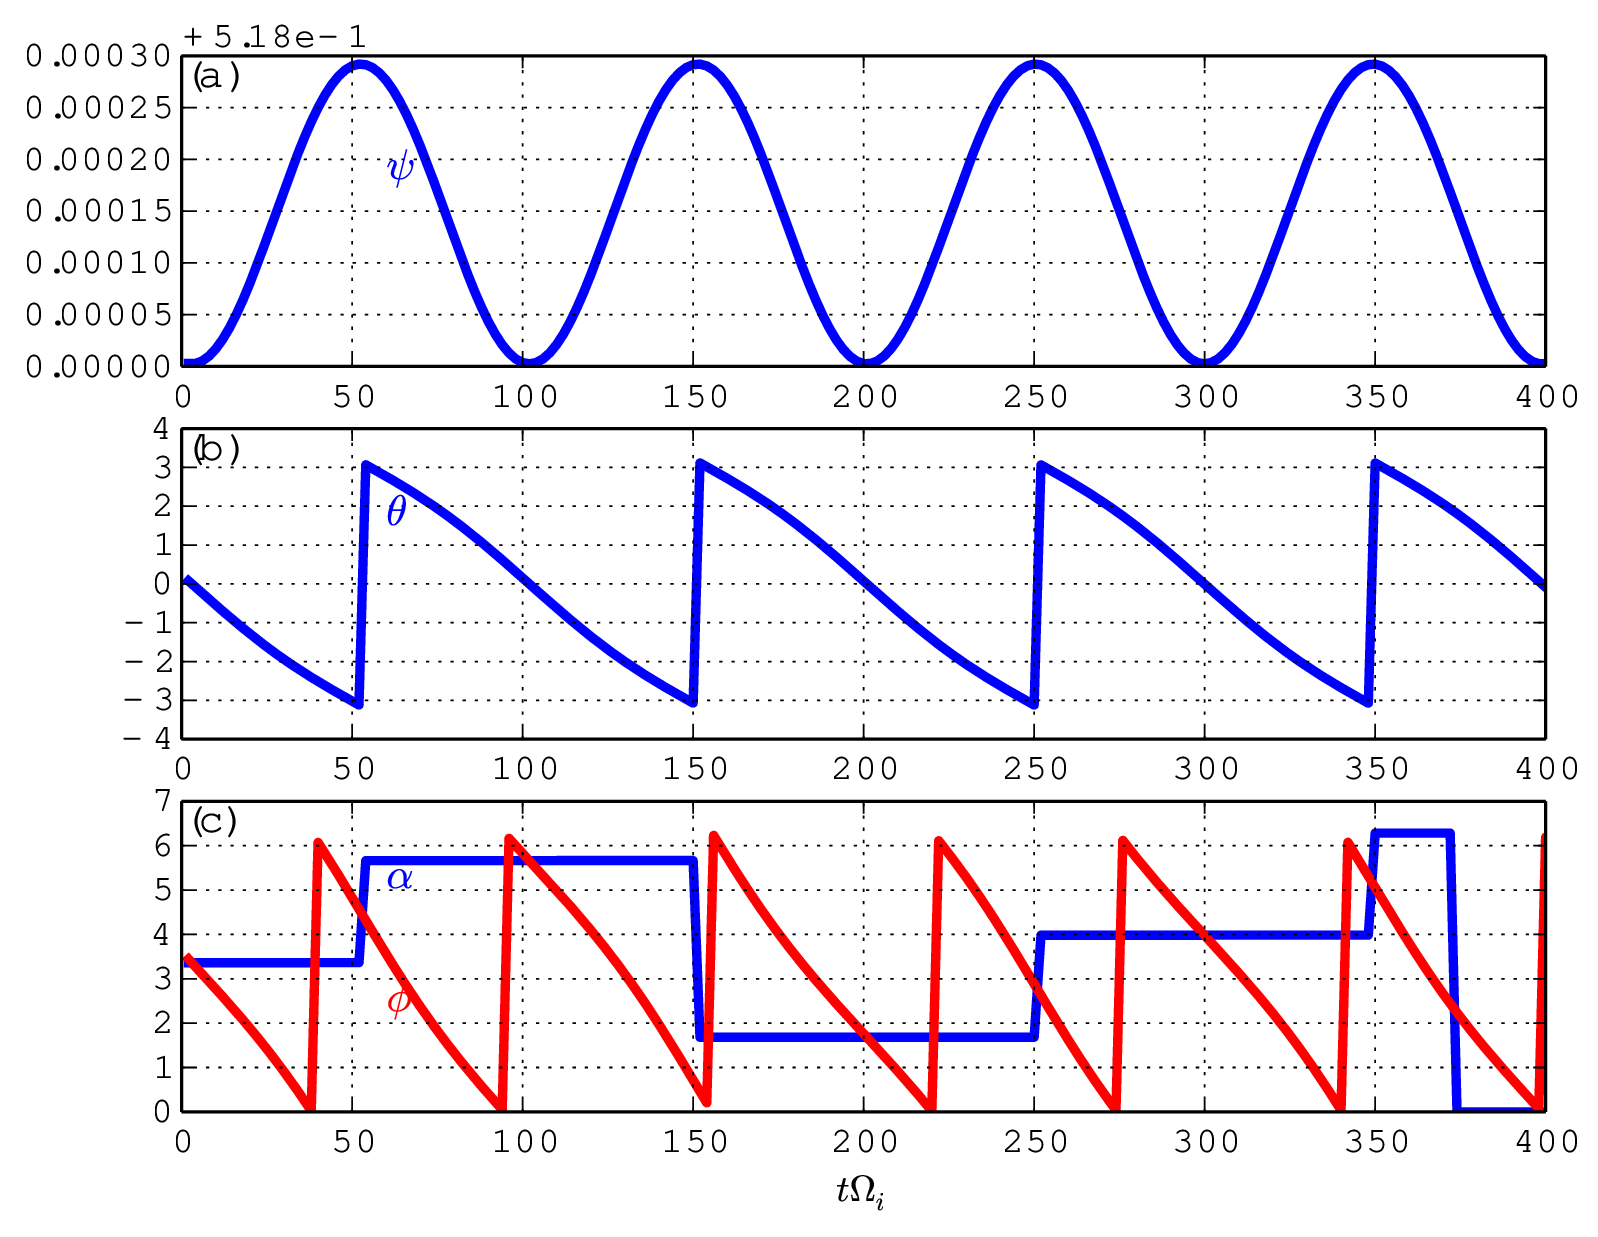
\includegraphics{/home/yj/project_new/test_space/sin_transform/f.eps}
  \caption{ \label{18-1-10-e1}The first five basis functions used in Fourier
  expansion (upper), sine expansion (middle), and cosine expansion (lower) in
  the interval $[x_0, x_0 + 2 L]$ with $x_0 = 0$ and $L = 1$.}
\end{figure}

\

The basis function $b_k (x)$ used in the Fourier expansion have the
properties $b_k (x) = b_k (x_0 + 2 L)$. Therefore Fourier expansion works best
for function that satisfy $h (x_0) = h (x_0 + 2 L)$. For a functions that do
not satisfies this condition, i.e., a function with $h (x_0) \neq h (x_0 + 2
L)$, the function can still be considered as a periodic function with period
$2 L$ but having discontinuity points at the interval boundary. It is well
known that Gibbs oscillations appear near discontinuity points, which can be
inner points in the interval or at the interval boundaries.

The basis functions $b_k (x)$ used in the sine expansion have the properties
$b_k (x_0) = b_k (x_0 + 2 L) = 0$. Therefore since expansion works best for
functions that satisfy $h (x_0) = h (x_0 + 2 L) = 0$. For functions that do
not satisfies this condition, there will be Gibbs oscillations near the
interval boundary when approximated by using the sine expansion. Examples are
shown in Fig. \ref{18-1-11-a1}.

The basis functions $b_k (x)$ used in the cosine expansion have the properties
$b_k' (x_0) = b_k' (x_0 + 2 L) = 0$. Therefore cosine expansion works best for
functions that satisfy $h' (x_0) = h' (x_0 + 2 L) = 0$. For functions that do
not satisfies this condition, there will be Gibbs oscillations near the
interval boundary when approximated by using the cosine expansion (to be
verified numerically by me).

\begin{figure}[h]
  \includegraphics{/home/yj/project_new/test_space/sin_transform/fig2/p.eps}\includegraphics{/home/yj/project_new/test_space/sin_transform/fig3/p.eps}
  \caption{\label{18-1-11-a1}Left: constant function $h (x) = 1$ approximated
  by using the sine expansion. Right: linear function $h (x) = x - 1$
  approximated by using the sine expansion. Gibbs oscillation appears near the
  boundaries, where $h (x)$ does not satisfy the condition $h (x_0) = h (x_0 +
  2 L) = 0$ ($x_0 = 0$ and $L = 1$ for this case). The expansion coefficients
  $H_k$ are obtained via the discrete sine transform (\ref{18-1-11-a2}) with
  number of sampling point $N = 50$. The reconstruction formula is given by $h
  (x) = \frac{2}{N} \sum_{k = 1}^{N - 1} H_k \sin ( \frac{k \pi x}{2 L}
  )$.}
\end{figure}

\

\

Next, let us discuss the sine and cosine transformation.

\subsection{Definition of the Discrete Sine Transform (DST)}

Figure (\ref{18-8-15-p3}) illustrates the grids used in the following
discussion.

\begin{figure}[h]
  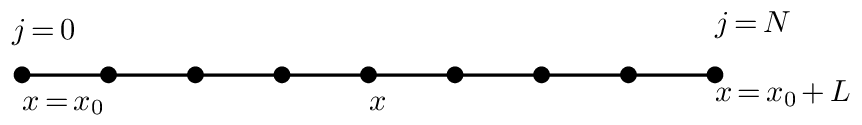
\includegraphics{/home/yj/theory/figures/sin_expansion/grids-2.eps}
  \caption{\label{18-8-15-p3}Grid indexes start from $0$ and ends at $N$. $h_0
  = h_N = 0$, i.e., $h (x_0) = h (x_0 + L) = 0$.}
\end{figure}

There are several slightly different types of Discrete Sine Transforms (DST).
One form I saw in W. Press's numerical recipe book is given by
\begin{equation}
  \label{18-1-11-a2} H_k = \sum_{j = 0}^{N - 1} h_j \sin \left( \frac{k \pi
  j}{N} \right),
\end{equation}
where $h_0 = h_N = 0$ are assumed. This form can be formally obtained by
replacing DFT's exponential function $\exp (2 \pi i k j / N)$ by $\sin (\pi k
j / N)$. The inverse sine transformation is given by (I did not derive this,
but had numerically verified that this transform recovers the original data if
applied after the sine transform (\ref{18-1-11-a2}) (code at
/home/yj/project\_new/test\_space/sine\_expansion/t2.f90))


\begin{equation}
  \label{18-8-15-p1} h_j = \frac{2}{N} \sum_{k = 0}^{N - 1} H_k \sin \left(
  \frac{k \pi j}{N} \right),
\end{equation}
which is identical with the forward sine transformation except for the
normalization factor $2 / N$. (The elements with index of zero can also be
excluded from the summation (\ref{18-1-11-a2}) and (\ref{18-8-15-p1}) since
these elements are zero). Replacing $j / N$ in Eq. (\ref{18-8-15-p1}) by $(x -
x_0) / L$ , we obtain the reconstructing function
\begin{equation}
  h (x) = \frac{2}{N} \sum_{k = 0}^{N - 1} H_k \sin \left( \frac{k \pi (x -
  x_0)}{L} \right) .
\end{equation}


\

We need a fast method of computing the above DST. All fast methods for this
finally need to make use of the fast method used in the computation of DFT. To
conveniently use the fast method of DFT, we need to define the DST in a way
that the DST can be easily connected to the DFT so that the DFT fast method
can be easily applied to compute the DST. A standard way of making this easy
is to define the DST via the DFT of an odd extension of the original data.
Next, let us discuss this.

\subsection{Define DST via DFT}

Let us introduce the Discrete Sine Transform (DST) by odd extending a given
real number sequence and then using the DFT of the extended data to define
DST. There are several slightly different way of odd extending a given
sequence and thus different types of DST. Given a $n = 3$ real number sequence
$(a, b, c)$, one frequently adopted odd extension is $(0, a, b, c, 0, - a, -
b, - c, 0)$. This odd extension is illustrated in Fig. \ref{18-1-11-e1}.

\begin{figure}[h]
  \resizebox{8cm}{!}{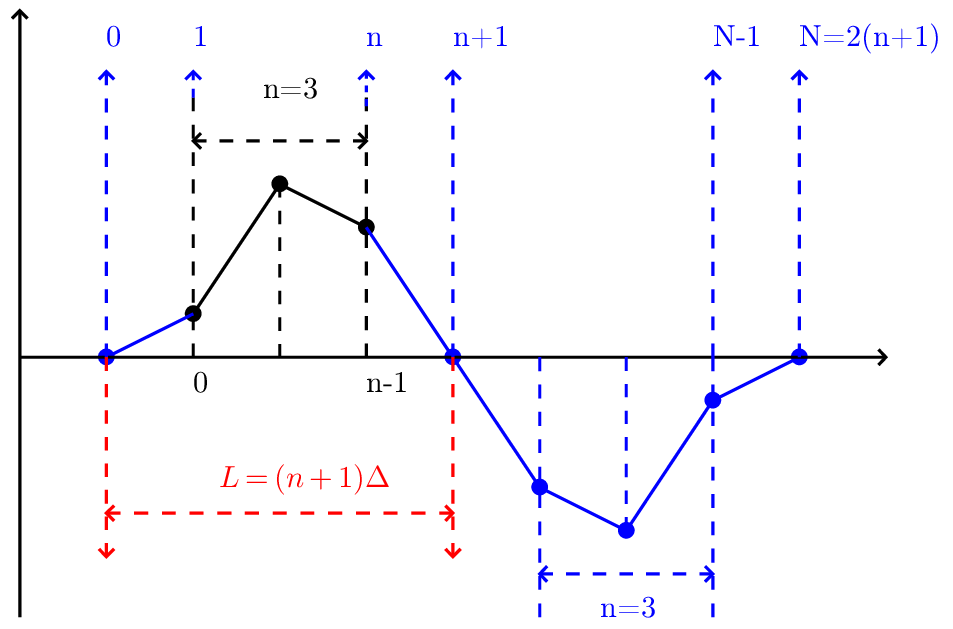
\includegraphics{/home/yj/theory/figures/odd_extension/t-1.eps}}
  \caption{\label{18-1-11-e1}A frequently used way of defining the odd
  extension of a sequence of real numbers . The black points are original data
  (with index $0, 1, \ldots, n - 1$). The blue points are newly introduced,
  together with the original points, generating an odd periodic sequence of
  numbers with index $0, 1, ., \ldots, N$, where $N = 2 (n + 1)$. The points
  used in the DFT are $0, 1, 2, \ldots, N - 1$. The period of these data is $2
  L$ with $L = (n + 1) \Delta$, where $\Delta$ is the spacing between points.}
\end{figure}

As illustrated in Fig. \ref{18-1-11-e1}, after the old extension, the total
number of points is $N + 1$ with $N = 2 (n + 1)$. Then DFT use the $N$ points
with index $j = 0, 1, \ldots, N - 1$ as input. Since the input are real and
odd symmetric sequence, the output of this DFT is an odd sequence of purely
imaginary numbers. Next, let us prove this. The DFT in this case is given by
\begin{equation}
  \label{18-1-12-a1} H_k = \sum_{j = 0}^{N - 1} h_j' \exp \left( - i \frac{2
  \pi k j}{N}  \right),
\end{equation}
where $h_j'$ is the odd extension of the original data $h_j$. For $j = 1, 2,
\ldots, n$, the relation between $h_j'$ and $h_j$ is given by
\begin{equation}
  \label{18-1-12-a2} h_j' = h_{j - 1},
\end{equation}
For $j = n + 2, \ldots, N - 1$, the relation is given by
\begin{equation}
  \label{18-1-12-a3} h_j' {= - h_{2 n + 1 - j}}  .
\end{equation}
Noting that $h_0' = 0$ and $h_{n + 1}' = 0$, then expression
(\ref{18-1-12-a1}) is written as
\begin{equation}
  H_k = 0 + \sum_{j = 1}^n h_j' \exp \left( - \frac{2 \pi i}{N} k j \right) +
  0 + \sum_{j = n + 2}^{N - 1} h_j' \exp \left( - \frac{2 \pi i}{N} k j
  \right) .
\end{equation}
Using $N = 2 (n + 1)$, the above expression is written as
\begin{equation}
  H_k = \sum_{j = 1}^n h_j' \exp \left( - \frac{\pi i}{(n + 1)} k j \right) +
  \sum_{j = n + 2}^{2 n + 1} h_j' \exp \left( - \frac{\pi i}{(n + 1)} k j
  \right)
\end{equation}
Using the relations (\ref{18-1-12-a2}) and (\ref{18-1-12-a3}) to replace
$h_j'$ by $h_j$, the above expression is written
\begin{equation}
  H_k = \sum_{j = 1}^n h_{j - 1} \exp \left( - \frac{\pi i}{(n + 1)} k j
  \right) - \sum_{j = n + 2}^{2 n + 1} h_{2 n + 1 - j} \exp \left( - \frac{\pi
  i}{(n + 1)} k j \right) .
\end{equation}
Change the definition of the dummy index $j$ in the above summation to make it
in the conventional range $[0 : n - 1]$, the above expression is written as
\[ H_k = \sum_{j = 0}^{n - 1} h_j \exp \left( - \frac{\pi i}{(n + 1)} k (j +
   1) \right) - \sum_{j = 0}^{n - 1} h_{n - 1 - j} \exp \left( - \frac{\pi
   i}{(n + 1)} k (j + n + 2) \right) . \]
Defining $j' = n - 1 - j$ to replace the dummy index in the second summation,
the above expression is written as
\begin{eqnarray}
  H_k & = & \sum_{j = 0}^{n - 1} h_j \exp \left( - \frac{\pi i}{(n + 1)} k (j
  + 1) \right) - \sum_{j' = n - 1}^0 h_{j'} \exp \left( - \frac{\pi i}{(n +
  1)} k (2 n + 1 - j') \right) . \nonumber\\
  & = & \sum_{j = 0}^{n - 1} h_j \exp \left( - \frac{\pi i}{(n + 1)} k (j +
  1) \right) - \sum_{j = 0}^{n - 1} h_j \exp \left( - \frac{\pi i}{(n + 1)} k
  (2 n + 1 - j) \right) . \nonumber\\
  & = & \sum_{j = 0}^{n - 1} h_j \exp \left( - \frac{\pi i}{(n + 1)} k (j +
  1) \right) - \sum_{j = 0}^{n - 1} h_j \exp \left( - \frac{\pi i}{(n + 1)} k
  (- j - 1) \right) . \nonumber\\
  & = & - 2 i \sum_{j = 0}^{n - 1} h_j \sin \left( \frac{\pi}{(n + 1)} k (j +
  1) \right),  \label{18-1-12-a6}
\end{eqnarray}
which is a purely imaginary number. Expression (\ref{18-1-12-a6}) also
indicates $H_k$ has the following symmetry
\begin{equation}
  \label{18-1-12-a8} H_{N - k} = - H_k,
\end{equation}
i.e. odd symmetry. Therefore only half of the data for $H_k$ with $k = 0, 1,
\ldots, N - 1$ need to be stored, namely $H_k$ with $k = 0, 1, \ldots, N / 2$.
Expression (\ref{18-1-12-a6}) indicates that $H_0$ and $H_{N / 2}$ are
definitely zero and thus do not need to be stored. Then the remaining data to
be stored are $H_k$ with $k = 1, 2, \ldots N / 2 - 1$, i.e. $k = 1, 2, \ldots,
n$. Following the convention of making the index of $H_k$ in the range $[0 : n
- 1]$, we define $H_k' = H_{k + 1}$. Then
\begin{equation}
  \label{18-1-12-a10} H_k' = - 2 i \sum_{j = 0}^{n - 1} h_j \sin \left(
  \frac{\pi}{(n + 1)}  (k + 1)  (j + 1) \right)
\end{equation}
with $k = 0, 1, 2, \ldots n - 1$, which is the index that we prefer. Finally,
the so-called type-I Discrete Sine Transform (DST-I) is defined based on Eq.
(\ref{18-1-12-a10}) via
\begin{equation}
  Y_k = \frac{H_k'}{- i} = 2 \sum_{j = 0}^{n - 1} h_j \sin \left(
  \frac{\pi}{(n + 1)}  (k + 1)  (j + 1) \right),
\end{equation}
with $k = 0, 1, 2, \ldots, n - 1$. This is the RODFT00 transform defined in
the FFTW library.

\subsection{Reconstruct original function using DST}

From the above derivation, we know that the DST, $Y_k$, is related to the DFT,
$H_k$, by $Y_k = H_{k + 1} / (- i)$, and thus the meaning of $Y_k$ is in
principle clear. Next, let us use the DST to reconstruct the original function
from which the data are sampled. Since DST is only a special case of DFT,
reconstructing the function using DST follows the same procedure used in DFT.
In DFT, the function is reconstructed via Eq. (\ref{11-9-1}) (changing to the
positive exponent convention), i.e.,
\begin{equation}
  \label{18-1-12-e1} h (x) = \frac{1}{N} \left[ \sum_{k = 0}^{N / 2} H_k \exp
  \left( i \frac{k 2 \pi x}{2 L} \right) + \sum_{k = N / 2}^{N - 1} H_k \exp
  \left( i \frac{(k - N) 2 \pi x}{2 L} \right) \right] .
\end{equation}
where $2 L$ is the length of the interval in which the samplings $h_j$ with $j
= 0, 1, \ldots, N - 1$ are made. For our present case, i.e., an odd extension
of the original $n$ data, we have $N = 2 (n + 1)$ and $H_0 = 0$ and $H_{N / 2}
= 0$. Then Eq. (\ref{18-1-12-e1}) is written as
\begin{equation}
  h (x) = \frac{1}{N} \left[ 0 + \sum_{k = 1}^n H_k \exp \left( i \frac{k 2
  \pi x}{2 L} \right) + 0 + \sum_{k = n + 2}^{2 n + 1} H_k \exp \left( i
  \frac{(k - N) 2 \pi x}{2 L} \right) \right] .
\end{equation}
Using the odd symmetry of $H_k$, i.e., $H_k = - H_{N - k}$, the above
expansion is written as
\begin{equation}
  h (x) = \frac{1}{N} \left[ \sum_{k = 1}^n H_k \exp \left( i \frac{k 2 \pi
  x}{2 L} \right) - \sum_{k = n + 2}^{2 n + 1} H_{N - k} \exp \left( i
  \frac{(k - N) 2 \pi x}{2 L} \right) \right] .
\end{equation}
Define $k' = 2 n + 2 - k$, and note that $N = 2 (n + 1)$, then the above
expression is written as
\begin{equation}
  h (x) = \frac{1}{2 (n + 1)} \left[ \sum_{k = 1}^n H_k \exp \left( i \frac{k
  2 \pi x}{2 L} \right) - \sum_{k' = n}^1 H_{k'} \exp \left( i \frac{(- k') 2
  \pi x}{2 L} \right) \right] .
\end{equation}
i.e.,
\begin{equation}
  h (x) = \frac{1}{2 (n + 1)} \sum_{k = 1}^n H_k \left[ \exp \left( i \frac{k
  2 \pi x}{2 L} \right) - \exp \left( - i \frac{k 2 \pi x}{2 L} \right)
  \right],
\end{equation}
which is simplified as
\begin{equation}
  \label{18-1-12-e3} h (x) = \frac{1}{2 (n + 1)} \sum_{k = 1}^n 2 i H_k \sin
  \left( \frac{k 2 \pi x}{2 L} \right) .
\end{equation}
As a convention, we prefer that the summation index begins from 0 and ends at
$n - 1$. Then expression (\ref{18-1-12-e3}) is written as
\[ h (x) = \frac{1}{2 (n + 1)} \sum_{k = 0}^{n - 1} 2 i H_{k + 1} \sin \left(
   \frac{(k + 1) 2 \pi x}{2 L} \right) \]
Using the relation between DST and DFT, i.e., $H_{k + 1} = - i Y_k$, the above
equation is written as
\begin{equation}
  \label{18-1-13-e3} h (x) = \frac{1}{n + 1} \sum_{k = 0}^{n - 1} Y_k \sin
  \left( \frac{(k + 1) 2 \pi x}{2 L} \right) .
\end{equation}
This is the formula for constructing the continuous function using the DST
data. This formula is an expansion over the basis functions $\sin [(k + 1) \pi
x / L]$ with the DST $Y_k$ acting as the expansion coefficients. Therefore the
direct meaning of the DST, $Y_k$, is that they are the expansion coefficients
when using $\sin (k \pi x / L)$ as the basis functions to approximate a
function in the domain $[0, L]$. From Fig. \ref{18-1-11-e1}, we know that the
interval length $L$ is given by $L = (n + 1) \Delta$, where $\Delta$ is the
uniform spacing between the original $n$ sampling points.

\subsubsection{Inverse DST}

Evaluate the function in Eq. (\ref{18-1-13-e3}) at $x_j = (j + 1) \Delta$ with
$j = 0, 1, \ldots, n - 1$, then we obtain
\begin{eqnarray}
  h (x_j) & = & \frac{1}{n + 1} \sum_{k = 0}^{n - 1} Y_k \sin \left( \frac{(k
  + 1) 2 \pi (j + 1) \Delta}{2 L} \right) \nonumber\\
  & = & \frac{1}{n + 1} \sum_{k = 0}^{n - 1} Y_k \sin \left( \frac{(k + 1)
  \pi (j + 1)}{(n + 1)} \right) .  \label{18-1-16-p1}
\end{eqnarray}
It can be proved that $h (x_j)$ in the above equation exactly recover $h_j$
used in defining the DST $Y_k$. Therefore Eq. (\ref{18-1-16-p1}) is the
Inverse Discrete Sine Transform.

\

\subsection{Discrete Cosine transform}

to be written

\section{Misc content}

\subsection{Nonlinear process}

The trigonometric identity
\begin{equation}
  2 \cos^2 (\omega t) = 1 + \cos (2 \omega t),
\end{equation}
indicates that nonlinear interaction between two waves of the same frequency
generates zero frequency component and its second harmonic. The process of
generating of second-harmonic is also called frequency doubling.

\subsection{Aliasing errors}

Signals that are not band-limited usually contains all frequencies and thus do
not satisfy the condition required by the sampling theorem (i.e., $H (f) = 0$
for $|f| > 1 / (2 \Delta)$). In this case, for any given $N$ data, we can
still calculate its DFT by using Eq. (\ref{2-26-2}). However the results
obtained are meaningful only when $H_n$ approaches zero as the frequency
approaches $- 1 / (2 \Delta)$ from above and approaches $1 / (2 \Delta)$ from
below, i.e., only when the results obtained are consistent with the assumption
used to obtain the results (the assumption is that $H (f) = 0$ for $|f| > 1 /
(2 \Delta)$). When the results obtained do not satisfy the above condition,
then it indicates that the ``aliasing errors'' have contributed to the
results. We can reduce the aliasing errors by increasing the sampling
frequency. The aliasing errors can be reduced but can not be completely
removed for a non-band-limited signal.

In signal processing and related disciplines, \tmtextbf{aliasing} is an effect
that causes different signals to become indistinguishable (or
\tmtextit{aliases} of one another) when sampled. It also often refers to the
distortion or artifact that results when a signal reconstructed from samples
is different from the original continuous signal.

An alias is a false lower frequency component that appears in sampled data
acquired at too low a sampling rate.

Aliasing errors are hard to detect and almost impossible to remove using
software. The solution is to use a high enough sampling rate, or if this is
not possible, to use an anti-aliasing filter in front of the analog-to-digital
converter (ADC) to eliminate the high frequency components before they get
into the data acquisition system.

When a digital image is viewed, a reconstruction is performed by a display or
printer device, and by the eyes and the brain. If the image data is processed
in some way during sampling or reconstruction, the reconstructed image will
differ from the original image, and an alias is seen.

\

Aliasing can be caused either by the sampling stage or the reconstruction
stage; these may be distinguished by calling sampling aliasing
(\tmtextit{prealiasing}) and reconstruction aliasing
(\tmtextit{postaliasing}).

In video or cinematography, temporal aliasing results from the limited frame
rate, and causes the
\href{https://en.wikipedia.org/wiki/Wagon-wheel\_effect}{wagon-wheel effect},
whereby a spoked wheel appears to rotate too slowly or even backwards.
Aliasing has changed its apparent frequency of rotation. A reversal of
direction can be described as a
\href{https://en.wikipedia.org/wiki/Negative\_frequency}{negative frequency}.
Temporal aliasing frequencies in video and cinematography are determined by
the frame rate of the camera, but the relative intensity of the aliased
frequencies is determined by the shutter timing (exposure time) or the use of
a temporal aliasing reduction filter during filming.

\subsection{Relation between Fourier series coefficients and DFTs}

In the above, we go through the process ``Fourier series$\rightarrow$Fourier
transformation $\rightarrow$DFT'', which corresponds to going from the
discrete case (Fourier series) to the continuous case (Fourier
transformation), and then back to the discrete case (DFT). Since both Fourier
series and DFT are discrete in frequency, it is instructive to examine the
relation between the Fourier coefficient $c_n$ and the DFT $H_n$. The Fourier
coefficient of $h (t)$ is given by Eq. (\ref{9-28-2}), i.e.,
\begin{equation}
  c_n = \frac{1}{T} \int_{- T / 2}^{T / 2} h (t) e^{i n 2 \pi t / T} d t,
\end{equation}
which can be equivalently written
\begin{equation}
  \label{9-29-3} c (f_n) = \frac{1}{T} \int_{- T / 2}^{T / 2} h (t) e^{i 2 \pi
  t f_n} d t,
\end{equation}
where $f_n = n / T$. On the other hand, if $h (t)$ is sampled with sampling
rate $f_s = 1 / \Delta$, then the number of sampling points per period is $N =
T / \Delta$. Then the frequency at which the Fourier transform $H (f)$ is
evaluated in getting the DFT [Eq. (\ref{10-26-1})] is written
\begin{equation}
  f_n = \frac{n}{\Delta N} = \frac{n}{T},
\end{equation}
which is identical to the frequency to which the Fourier coefficient $c_n$
corresponds. Using $f_n = n / (\Delta N)$ in Eq. (\ref{9-29-3}), we obtain
\begin{eqnarray}
  c (f_n) & = & \frac{1}{T} \int_{- T / 2}^{T / 2} h (t) \exp \left( \frac{i 2
  \pi t n}{\Delta N} \right) d t. \nonumber\\
  & \approx & \frac{1}{T} \Delta \sum_{j = 0}^{N - 1} h_j \exp \left( \frac{2
  \pi i}{N} n j \right)  \label{10-6-e1}\\
  & = & \frac{1}{T} \Delta H_n \nonumber\\
  & = & \frac{1}{N} H_n 
\end{eqnarray}
i.e., dividing the DFT $H_n$ by $N$ gives the corresponding Fourier expansion
coefficient $c_n$. We can further use Eqs. (\ref{18-2-2p1}) and
(\ref{18-2-2p2}) to recover the Fourier coefficients in terms of trigonometric
functions cosine and sine,

Note that the approximation in Eq. (\ref{10-6-e1}) becomes an exact relation
if the largest frequency contained in $h (t)$ is less than $1 / (2 \Delta)$.

\appendix\section{Efficient method of computing DFT: Fast Fourier
Transformation (FFT) algorithm (not
finished)}\label{23-3-23-p1}\label{18-1-28-a1}

The DFT is defined by Eq. (\ref{2-26-2}), i.e.,
\begin{equation}
  \label{18-1-28-a2} H_j \equiv \sum_{k = 0}^{N - 1} W^{k j} h_k,
\end{equation}
where $W = \exp (2 \pi i / N)$. Equations (\ref{18-1-28-a2}) indicates that
the DFT is the multiplication of a transformation matrix $M_{k j} \equiv W^{k
j}$ with a column vector $h_k$, where the transformation matrix $M_{k j}$ is
symmetric and called DFT matrix. In the matrix form, the DFT is written as
\begin{equation}
  \label{18-1-31-a1} \left(\begin{array}{c}
    H_1\\
    H_2\\
    H_3\\
    H_4\\
    \vdots\\
    H_{N - 1}
  \end{array}\right) = \left(\begin{array}{cccccc}
    1 & 1 & 1 & 1 & \ldots & 1\\
    1 & W^1 & W^2 & W^3 & \ldots & W^{N - 1}\\
    1 & W^2 & W^4 & W^6 & \ldots & W^{2 (N - 1)}\\
    1 & W^3 & W^6 & W^9 & \ldots & W^{3 (N - 1)}\\
    \vdots & \vdots & \vdots & \vdots & \ddots & \vdots\\
    1 & W^{N - 1} & W^{2 (N - 1)} & W^{3 (N - 1)} & \ldots & W^{(N - 1) (N -
    1)}
  \end{array}\right) \left(\begin{array}{c}
    h_1\\
    h_2\\
    h_3\\
    h_4\\
    \vdots\\
    h_{N - 1}
  \end{array}\right)
\end{equation}
If directly using the definition in Eq. (\ref{18-1-31-a1}) to compute DFT,
then a matrix multiplication need to be performed, which requires $O (N^2)$
operations. Here the powers of $W$ are assumed to be pre-computed, and we
define ``an operation'' as a multiplication followed by an addition.

\

The Fast Fourier Transformation (FFT) algorithm manage to reduce the
complexity of computing the DFT from $O (N^2)$ to $O (N \log_2 N)$ by
factoring the DFT matrix $M_{k j}$ into a product of sparse matrices.

The original paper on FFT is Cooley and Tukey's paper: An algorithm for the
machine calculation of complex Fourier series, which turns out to be a very
concise paper.

Suppose $N$ is a composite, i.e., $N = r_1 \cdot r_2$. Then the indices in Eq.
(\ref{18-1-28-a2}) can be expressed as
\begin{equation}
  j = j_1 r_1 + j_0, \hspace{2.6em} j_0 = 0, 1, \ldots, r_1 - 1,
  \hspace{2.2em} j_1 = 0, 1, \ldots, r_2 - 1
\end{equation}
\begin{equation}
  k = k_1 r_2 + k_0, \hspace{2.0em} k_0 = 0, 1, \ldots, r_2 - 1,
  \hspace{2.0em} k_1 = 0, 1, \ldots, r_1 - 1
\end{equation}
Then, one can write
\begin{equation}
  H (j_0, j_1) = \sum_{k_0} \sum_{k_1} h (k_0, k_1) W^{(j k_1 r_2 + j k_0)},
\end{equation}
Noting that
\begin{equation}
  W^{j k_1 r_2} = W^{j_1 r_1 k_1 r_2 + j_0 k_1 r_2} = W^{j_0 k_1 r_2}
\end{equation}
Eq. () is written as
\begin{equation}
  H (j_0, j_1) = \sum_{k_0} \left( \sum_{k_1} h (k_0, k_1) W^{(j_0 k_1 r_2)}
  \right) W^{(j k_0)},
\end{equation}
where the inner sum over $k_1$ is independent of $j_1$ and can be defined as a
new array
\begin{equation}
  h_1 (j_0, k_0) = \sum_{k_1} h (k_0, k_1) W^{(j_0 k_1 r_2)} .
\end{equation}
Then
\begin{equation}
  H (j_0, j_1) = \sum_{k_0} h_1 (j_0, k_0) W^{(j_1 r_1 + j_0) k_0},
\end{equation}
There are $N$ elements in the array $h_1$, each requiring $r_1$ operations,
giving a total of $N r_1$ operation to obtain $h_1$. Similarly, it takes $N
r_2$ operations to calculate $H$ from $h_1$. Therefore, this two-step
algorithm requires a total of $N (r_1 + r_2)$ operations.

\

\section{Fourier series$\rightarrow$Fourier transformation}

\subsection{From discrete spectrum to continuous spectrum}

The Fourier series discussed above indicates that a periodic function is
composed of discrete spectrum and is written as
\begin{equation}
  \label{9-27-e14} h (t) = \sum_{n = - \infty}^{\infty} c_n \exp \left( i
  \frac{n 2 \pi}{T} t \right) ,
\end{equation}
where $T$ is the period of $h (t)$. The $n$th term of the above Fourier series
corresponds to a harmonic of frequency
\begin{equation}
  \label{9-27-e10} f_n = \frac{n}{T},
\end{equation}
and the expansion coefficient $c_n$ is given by
\begin{equation}
  \label{9-28-2} c_n = \frac{1}{T} \int_{- T / 2}^{T / 2} h (t) \exp \left( -
  i \frac{n 2 \pi}{T} t \right) d t.
\end{equation}
In terms of $f_n$, the coefficient in Eq. (\ref{9-28-2}) is written
\begin{equation}
  \label{9-27-e11} c_n = c (f_n) = \frac{1}{T} \int_{- T / 2}^{T / 2} h (t)
  \exp (- i 2 \pi f_n t)  d t
\end{equation}
In terms of $f_n$, the Fourier series in Eq. (\ref{9-27-e14}) is written
\begin{eqnarray}
  h (t) & = & \sum_{n = - \infty}^{\infty} c (f_n) e^{i 2 \pi t f_n}
  \nonumber\\
  & = & T \sum_{n = - \infty}^{\infty} c (f_n) e^{i 2 \pi t f_n} \frac{1}{T} 
  \label{9-28-5}
\end{eqnarray}
Note that $c (f_n) e^{i 2 \pi t f_n}$ is the value of function $c (f) e^{i 2
\pi t f}$ at $f = f_n$. Further note that the interval between $f_n$ and $f_{n
+ 1}$ is $1 / T$. Thus the above summation is the rectangular formula for
numerically calculating the integration $\int_{- \infty}^{\infty} c (f) e^{i 2
\pi t f} d f$. Therefore, equation (\ref{9-28-5}) can be approximately written
as
\begin{equation}
  h (t) \approx T \int_{- \infty}^{\infty} c (f) e^{i 2 \pi t f} d f,
\end{equation}
which will become exact when the interval $1 / T \rightarrow 0$, i.e., $T
\rightarrow \infty$. Therefore, for the case $T \rightarrow \infty$, the
Fourier series exactly becomes
\begin{equation}
  \label{9-28-6} h (t) = T \int_{- \infty}^{\infty} c (f) e^{i 2 \pi t f} d f,
\end{equation}
where $c (f)$ is given by Eq. (\ref{9-27-e11}), i.e.,
\begin{equation}
  \label{9-28-7} c (f) = \frac{1}{T} \int_{- T / 2}^{T / 2} h (t) e^{- i 2 \pi
  t f} d t.
\end{equation}
Note that the function $h (t)$ given in Eq. (\ref{9-28-6}) is proportional to
$T c (f)$ while the function $c (f)$ given in Eq. (\ref{9-28-7}) is
proportional to $1 / T$. Since $T \rightarrow \infty$, it is desired to
eliminate the $T$ and $1 / T$ factors in Eqs. (\ref{9-28-6}) and
(\ref{9-28-7}), which can be easily achieved by defining a new function
\begin{equation}
  H (f) = T c (f) .
\end{equation}
Then equations (\ref{9-28-6}) and (\ref{9-28-7}) are written as
\begin{equation}
  \label{9-28-10} h (t) = \int_{- \infty}^{\infty} H (f) e^{i 2 \pi t f} d f,
\end{equation}
\begin{equation}
  \label{9-28-11} H (f) = \int_{- T / 2}^{T / 2} h (t) e^{- i 2 \pi t f} d t =
  \int_{- \infty}^{\infty} h (t) e^{- i 2 \pi t f} d t,
\end{equation}
Equations (\ref{9-28-10}) and (\ref{9-28-11}) are the Fourier transformation
pairs discussed in the next section.

\subsection{Fourier transformation}

As discussed above, the Fourier transformation of a function $h (t)$ is given
by
\begin{equation}
  \label{10-3-e1} H (f) = \int_{- \infty}^{\infty} h (t) e^{i 2 \pi f t} d t.
\end{equation}
Once the Fourier transformation $H (f)$ is known, the original function $h
(t)$ can be reconstructed via
\begin{equation}
  \label{10-11-3} h (t) = \int_{- \infty}^{\infty} H (f) e^{- i 2 \pi f t} d
  f.
\end{equation}


[Note that the signs in the exponential of Eq. (\ref{9-28-10}) and
(\ref{9-28-11}) are opposite. Which one should be minus or positive is
actually a matter of convention because a trivial variable substitution $f' =
- f$ can change the sign between minus and positive. Proof. In terms of $f'$,
Eq. \ (\ref{10-11-3}) is written
\begin{eqnarray}
  h (t) & = & \int_{\infty}^{- \infty} H (- f') e^{i 2 \pi t f'} d (- f'),
  \nonumber\\
  & = & \int_{- \infty}^{\infty} H (- f') e^{i 2 \pi t f'} d f', 
  \label{9-28-23}
\end{eqnarray}
Define
\begin{eqnarray}
  \overline{H} (f') & \equiv & H (- f') \nonumber\\
  & = & \int_{- \infty}^{\infty} h (t) e^{- i 2 \pi t f'} d t. 
  \label{9-28-20}
\end{eqnarray}
Then Eq. (\ref{9-28-23}) is written
\begin{equation}
  \label{9-28-21} h (t) = \int_{- \infty}^{\infty} \overline{H} (f') e^{i 2
  \pi t f'} d f'
\end{equation}
The signs in the exponential of Eqs. (\ref{9-28-20}) and (\ref{9-28-21}) are
opposite to Eqs. (\ref{10-3-e1}) and (\ref{10-11-3}), respectively.]

[Some physicists prefer to use the angular frequency $\omega \equiv 2 \pi f$
rather than the frequency $f$ to represent the Fourier transformation. Using
$\omega$, equations. (\ref{10-3-e1}) and (\ref{10-11-3}) are written,
respectively, as
\begin{equation}
  H (\omega) = \int_{- \infty}^{\infty} h (t) e^{i \omega t} d t,
\end{equation}
\begin{equation}
  h (t) = \frac{1}{2 \pi} \int_{- \infty}^{\infty} H (\omega) e^{- i \omega t}
  d \omega,
\end{equation}
where we see that the asymmetry between the Fourier transformation and its
inverse is more severe in this representation: besides the opposite-sign in
the exponents, there is also a $1 / 2 \pi$ factor difference between the
Fourier transformation and its inverse. Whether the $1 / 2 \pi$ factor appears
at the forward transformation or inverse one is actually a matter of
convention. The only requirement is that the product of the two factors in the
forward and inverse transformation is equal to $1 / 2 \pi$. To obtain a more
symmetric pair, one can adopt a factor $1 / \sqrt{2 \pi}$ at both the forward
and inverse transformation. The representation in Eqs. (\ref{10-3-e1}) and
(\ref{10-11-3}) is adopted in this note. But we should know how to change to
the $\omega$ representation when needed.]

[
\begin{equation}
  \int_{- \infty}^{\infty} \frac{d h (t)}{d t} e^{- i 2 \pi t f} d t = h (t)
  e^{- i 2 \pi t f} |_{- \infty}^{+ \infty} \nobracket - \int_{-
  \infty}^{\infty} h (t) \frac{d e^{- i 2 \pi t f}}{d t} d t = - \int_{-
  \infty}^{\infty} h (t) \frac{d e^{- i 2 \pi t f}}{d t} d t = i 2 \pi f
  \int_{- \infty}^{\infty} h (t) e^{- i 2 \pi t f} d t = i 2 \pi f H (f)
\end{equation}
]

\subsection{Numerical computation of Fourier transformation}

Next, consider how to numerically compute the Fourier transformation of a
function $h (t)$. A simple way is to use the rectangle formula to approximate
the integration in Eq. (\ref{10-3-e1}), i.e.,
\begin{equation}
  \label{10-3-e2} H (f) \approx \Delta \sum_{j = - \infty}^{\infty} h_j \exp
  (i 2 \pi f j \Delta),
\end{equation}
where $h_j = h (t_j)$ and $t_j = j \Delta$ with $j = \ldots, - 2, - 1, 0, 1,
2, \ldots$. Note Eq. (\ref{10-3-e2}) is an approximation, which will become
exact if $\Delta \rightarrow 0$. In practice, we can sample $h (t)$ only with
a nonzero $\Delta$. Therefore Eq. (\ref{10-3-e2}) is usually an approximation.
Do we have some rules to choose a suitable $\Delta$ so that Eq.
(\ref{10-3-e2}) can become a good approximation or even an exact relation?
This important question is answered by the sampling theorem, which sates that
a suitable $\Delta$ to make Eq. (\ref{10-3-e2}) exact is given by $\Delta
\leqslant 1 / (2 f_c)$, where $f_c$ is the largest frequency contained in $h
(t)$ (i.e., $H (f) = 0$ for $|f| > f_c$).

\subsection{Sampling theorem}

In computational and experimental work, we know only a list of values $h
(t_j)$ sampled at discrete values of $t_j$. Let us suppose that $h (t)$ is
sampled with uniform interval between consecutive points:
\begin{equation}
  h_j = h (t_j), t_j = j \Delta, j = \ldots, - 2, - 1, 0, 1, 2, \ldots
\end{equation}
The sampling rate is defined by $f_s = 1 / \Delta$. The sampling theorem
states that: If the Fourier transformation of function $h (t)$, $H (f)$, has
the following property
\begin{equation}
  \label{8-28-3} H (f) = 0 \tmop{for} |f| \geqslant f_c
\end{equation}
then sampling $h (t)$ with the sampling rate $f_s \geqslant 2 f_c$ (i.e.,
$\Delta \leqslant 1 / (2 f_c)$) will completely determine $h (t)$, which is
given explicitly by the formula
\begin{equation}
  \label{8-28-4} h (t) = \Delta \sum_{j = - \infty}^{\infty} h_j \frac{\sin [2
  \pi f_c (t - j \Delta)]}{\pi (t - j \Delta)} .
\end{equation}
We will not concern us here with the proof of the sampling theorem and simply
start working with Eq. (\ref{8-28-4}) to derive the concrete expression for
the Fourier transformation of $h (t)$. Substituting the expression
(\ref{8-28-4}) for $h (t)$ into the Fourier transformation (\ref{10-3-e1}), we
obtain the explicit form of the Fourier transformation of $h (t)$:
\begin{eqnarray}
  H (f) & \equiv & \int_{- \infty}^{\infty} h (t) \exp (i 2 \pi f t) d t,
  \nonumber\\
  & = & \Delta \sum_{j = - \infty}^{\infty} h_j \int_{- \infty}^{\infty}
  \frac{\sin [2 \pi f_c (t - j \Delta)]}{\pi (t - j \Delta)} \exp (i 2 \pi f
  t) d t, \nonumber\\
  & = & \Delta \sum_{j = - \infty}^{\infty} h_j \exp (i 2 \pi f j \Delta)
  \int_{- \infty}^{\infty} \frac{\sin [2 \pi f_c (t - j \Delta)]}{\pi (t - j
  \Delta)} \exp [i 2 \pi f (t - j \Delta)] d t, \nonumber\\
  & = & \Delta \sum_{j = - \infty}^{\infty} h_j \exp (i 2 \pi f j \Delta)
  \int_{- \infty}^{\infty} \frac{\sin [2 \pi f_c \tau]}{\pi \tau} \exp [i 2
  \pi f \tau] d \tau .  \label{8-28-1}
\end{eqnarray}
With the help of Wolfram Mathematica, the integration in Eq. (\ref{8-28-1}) is
evaluated analytically, giving
\begin{equation}
  \int_{- \infty}^{\infty} \frac{\sin [2 \pi f_c \tau]}{\pi \tau} \exp (i 2
  \pi f \tau) d \tau = \left\{ \begin{array}{l}
    0 \tmop{For} |f| > f_c\\
    1 \tmop{For} |f| < f_c
  \end{array} . \right.
\end{equation}
Using this, \ Eq. (\ref{8-28-1}) is written
\begin{equation}
  \label{8-28-5} H (f) = \left\{ \begin{array}{l}
    0 \tmop{for} |f| > f_c\\
    \Delta \sum_{j = - \infty}^{\infty} h_j \exp (i 2 \pi f j \Delta)
    \tmop{for} |f| \leqslant f_c
  \end{array}, \right.
\end{equation}
which shows that $H (f) = 0$ for $|f| > f_c$, which is consistent with the
assumption of sampling theorem, i.e., $H (f)$ has the property given in Eq.
(\ref{8-28-3}). The second line of Eq. (\ref{8-28-5}) is identical to Eq.
(\ref{10-3-e2}) except that Eq. (\ref{8-28-5}) in this case is exact while Eq.
(\ref{10-3-e2}) is only approximate. In other words, if $\Delta \leqslant 1 /
(2 f_c)$, then the Fourier transformation is exactly given by Eq.
(\ref{8-28-5}), where $f_c$ is the largest frequency contained in $h (t)$
(i.e., $H (f) = 0$ for $|f| > f_c$).

\section{Multi-dimensional Fourier series}

\subsection{2D Fourier series in terms of complex basis functions}

Compared with Eq. (\ref{2-25-1}) that uses the trigonometric functions,
Fourier series (\ref{2-25-p6}) and (\ref{2-25-p7}), which is expressed in
terms of the complex exponential function $e^{i n \pi x / L}$, is more
compact. The convenience introduced by the complex exponential function is
more obvious when we deal with multiple-dimensional cases. For example, a
two-dimensional function $G (x, y)$ can be expanded as Fourier series about
$x$,
\begin{equation}
  \label{10-22-p2} G (x, y) = \sum_{m = - \infty}^{\infty} c_m (y) e^{i m \pi
  x / L_x},
\end{equation}
where $2 L_x$ is the period of $G$ in $x$ direction. The expansion
coefficients $c_m (y)$ can be further expanded as Fourier series about $y$,
\begin{equation}
  \label{10-22-p1} c_m (y) = \sum_{n = - \infty}^{\infty} (c_{m n} e^{i n \pi
  y / L_y}),
\end{equation}
where $2 L_y$ is the period of $G$ in $y$ direction, and the coefficients
$c_{m n}$ is given by
\begin{eqnarray}
  c_{m n} & = & \frac{1}{2 L_y} \int_{- L_y}^{L_y} \left[ \frac{1}{2 L_x}
  \int_{- L_x}^{L_x} G (x, y) e^{- i m \pi x / L_x} d x \right] e^{- i n \pi y
  / L_y} d y. \nonumber\\
  & = & \frac{1}{4 L_x L_y} \int_{- L_y}^{L_y} \int_{- L_x}^{L_x} G (x, y)
  {e^{- i m \pi x / L_x - i n \pi y / L_y}}  d x d y.  \label{2-4-1}
\end{eqnarray}
Using Eq. (\ref{10-22-p1}) in Eq. (\ref{10-22-p2}), we obtain
\begin{equation}
  \label{10-22-e1} G (x, y) = \sum_{m = - \infty}^{\infty} \sum_{n = -
  \infty}^{\infty} c_{m n} e^{i n \pi y / L_y + i m \pi x / L_x},
\end{equation}
Equations (\ref{10-22-e1}) and (\ref{2-4-1}) give the two-dimensional Fourier
series of $G (x, y)$.

The formula for expanding a real-valued two-dimensional function $G (x, y)$ in
terms of basis functions $\cos \left( \frac{m \pi x}{L_x} + \frac{n \pi
y}{L_y} \right)$ and $\sin \left( \frac{m \pi x}{L_x} + \frac{n \pi y}{L_y}
\right)$ can be readily recovered from Eqs. (\ref{10-22-e1}) and
(\ref{2-4-1}). For notation ease, define
\begin{equation}
  \alpha = \frac{m \pi x}{L_x} + \frac{n \pi y}{L_y} .
\end{equation}
Then Eq. (\ref{10-22-e1}) is written as
\begin{eqnarray*}
  G (x, y) & = & \sum_{m = - \infty}^{\infty} \sum_{n = - \infty}^{\infty}
  c_{m n} [\cos \alpha + i \sin \alpha]\\
  & = & \sum_{m = - \infty}^{\infty} \sum_{n = - \infty}^{\infty} \left(
  \frac{1}{4 L_x L_y} \int_{- L_y}^{L_y} \int_{- L_x}^{L_x} G (x, y) \cos
  \alpha d x d y \right)  [\cos \alpha + i \sin \alpha]\\
  & + & \sum_{m = - \infty}^{\infty} \sum_{n = - \infty}^{\infty} \left(
  \frac{1}{4 L_x L_y} \int_{- L_y}^{L_y} \int_{- L_x}^{L_x} G (x, y) \sin
  \alpha d x d y \right) [- i \cos \alpha + \sin \alpha],
\end{eqnarray*}
Sine $G (x, y)$ is assumed to be real-valued, the imaginary parts of the above
expression will cancel each other. Therefore, the above expansion is
simplified to
\begin{eqnarray}
  G (x, y) & = & \sum_{m = - \infty}^{\infty} \sum_{n = - \infty}^{\infty}
  \left( \frac{1}{4 L_x L_y} \int_{- L_y}^{L_y} \int_{- L_x}^{L_x} G (x, y)
  \cos \alpha d x d y \right) \cos \alpha \nonumber\\
  & + & \sum_{m = - \infty}^{\infty} \sum_{n = - \infty}^{\infty} \left(
  \frac{1}{4 L_x L_y} \int_{- L_y}^{L_y} \int_{- L_x}^{L_x} G (x, y) \sin
  \alpha d x d y \right) \sin \alpha .  \label{23-3-31-p1}
\end{eqnarray}


\subsection{2D Fourier series using trigonometric functions cosine and
sine}\label{10-23-8}

We see that the extension of Fourier series from one-dimension case to
two-dimension case is straightforward when expressed in terms of the complex
exponential function $e^{i n \pi x / L}$. However, if we use $\sin (m \pi x /
L_x)$, $\cos (m \pi x / L_x)$, $\sin (n \pi y / L_y)$, and $\cos (n \pi y /
L_y)$ as basis functions, the derivation of the two-dimensional Fourier series
of $G (x, y)$ is a little complicated (product-to-sum trigonometric identities
are involved to simplify the results).

In this section, we derive the two-dimensional Fourier series using cosine and
sine as basis functions. A two-dimensional function $G (x, y)$ can be first
expanded as Fourier series about $x$,
\begin{equation}
  \label{10-23-3} G (x, y) = \sum_{m = 1}^{\infty} a_m (y) \cos \left( \frac{m
  \pi}{L_x} x \right) + \sum_{m = 1}^{\infty} b_m (y) \sin \left( \frac{m
  \pi}{L_x} x \right),
\end{equation}
(the zero-frequency component is dropped, will take it back later) and then
the two coefficients $a_m (y)$ and $b_m (y)$ can be further expanded as
Fourier series about $y$,
\begin{equation}
  \label{10-23-1} a_m (y) = \sum_{n = 1}^{\infty} a_{m n}^{(a)} \cos \left(
  \frac{n \pi}{L_y} y \right) + \sum_{n = 1}^{\infty} b_{m n}^{(a)} \sin
  \left( \frac{n \pi}{L_y} y \right),
\end{equation}
\begin{equation}
  \label{10-23-2} b_m (y) = \sum_{n = 1}^{\infty} a_{m n}^{(b)} \cos \left(
  \frac{n \pi}{L_y} y \right) + \sum_{n = 1}^{\infty} b_{m n}^{(b)} \sin
  \left( \frac{n \pi}{L_y} y \right),
\end{equation}
(the zero-frequency component is dropped, will take it back later)
Substituting Eq. (\ref{10-23-1}) and (\ref{10-23-2}) into Eq. (\ref{10-23-3}),
we obtain
\begin{eqnarray}
  G (x, y) & = & \sum_{m = 1}^{\infty} \left[ \sum_{n = 1}^{\infty} a_{m
  n}^{(a)} \cos \left( \frac{n \pi}{L_y} y \right) + \sum_{n = 1}^{\infty}
  b_{m n}^{(a)} \sin \left( \frac{n \pi}{L_y} y \right) \right] \cos \left(
  \frac{m \pi}{L_x} x \right) \nonumber\\
  & + & \sum_{m = 1}^{\infty} \left[ \sum_{n = 1}^{\infty} a_{m n}^{(b)} \cos
  \left( \frac{n \pi}{L_y} y \right) + \sum_{n = 1}^{\infty} b_{m n}^{(b)}
  \sin \left( \frac{n \pi}{L_y} y \right) \right] \sin \left( \frac{m
  \pi}{L_x} x \right) .  \label{10-23-4}
\end{eqnarray}
Using the product-to-sum trigonometric identities, equation (\ref{10-23-4}) is
written
\begin{eqnarray*}
  G (x, y) & = & \frac{1}{2} \sum_{m = 1}^{\infty} \sum_{n = 1}^{\infty} a_{m
  n}^{(a)} \left[ \cos \left( \frac{m \pi}{L_x} x + \frac{n \pi}{L_y} y
  \right) + \cos \left( \frac{m \pi}{L_x} x - \frac{n \pi}{L_y} y \right)
  \right]\\
  & + & \frac{1}{2} \sum_{m = 1}^{\infty} \sum_{n = 1}^{\infty} b_{m n}^{(a)}
  \left[ \sin \left( \frac{m \pi}{L_x} x + \frac{n \pi}{L_y} y \right) + \sin
  \left( \frac{m \pi}{L_x} x - \frac{n \pi}{L_y} y \right) \right]\\
  & + & \frac{1}{2} \sum_{m = 1}^{\infty} \sum_{n = 1}^{\infty} a_{m n}^{(b)}
  \left[ \sin \left( \frac{m \pi}{L_x} x + \frac{n \pi}{L_y} y \right) - \sin
  \left( \frac{m \pi}{L_x} x - \frac{n \pi}{L_y} y \right) \right]\\
  & + & \frac{1}{2} \sum_{m = 1}^{\infty} \sum_{n = 1}^{\infty} b_{m n}^{(b)}
  \left[ \cos \left( \frac{m \pi}{L_x} x - \frac{n \pi}{L_y} y \right) - \cos
  \left( \frac{m \pi}{L_x} x + \frac{n \pi}{L_y} y \right) \right]
\end{eqnarray*}
which can be organized as
\begin{eqnarray}
  G (x, y) & = & \sum_{m = 1}^{\infty} \sum_{n = 1}^{\infty} \frac{1}{2} [a_{m
  n}^{(a)} - b_{m n}^{(b)}] \cos \left( \frac{m \pi}{L_x} x + \frac{n
  \pi}{L_y} y \right) \nonumber\\
  & + & \sum_{m = 1}^{\infty} \sum_{n = 1}^{\infty} \frac{1}{2} [b_{m
  n}^{(a)} + a_{m n}^{(b)}] \sin \left( \frac{m \pi}{L_x} x + \frac{n
  \pi}{L_y} y \right) \nonumber\\
  & + & \sum_{m = 1}^{\infty} \sum_{n = 1}^{\infty} \frac{1}{2} [a_{m
  n}^{(a)} + b_{m n}^{(b)}] \cos \left( \frac{m \pi}{L_x} x - \frac{n
  \pi}{L_y} y \right) \nonumber\\
  & + & \sum_{m = 1}^{\infty} \sum_{n = 1}^{\infty} \frac{1}{2} [b_{m
  n}^{(a)} - a_{m n}^{(b)}] \sin \left( \frac{m \pi}{L_x} x - \frac{n
  \pi}{L_y} y \right)  \label{11-9-4}
\end{eqnarray}
The coefficients appearing above are written as
\begin{equation}
  a_m (y) = \frac{1}{L_x} \int_{- L_x}^{- L_x} G (x, y) \cos \left( \frac{m
  \pi}{L_x} x \right) d x
\end{equation}
\begin{equation}
  b_m (y) = \frac{1}{L_x} \int_{- L_x}^{- L_x} G (x, y) \sin \left( \frac{m
  \pi}{L_x} x \right) d x
\end{equation}

\begin{equation}
  a_{m n}^{(a)} = \frac{1}{L_x}  \frac{1}{L_y} \int_{- L_y}^{- L_y} \int_{-
  L_x}^{- L_x} G (x, y) \cos \left( \frac{m \pi}{L_x} x \right) \cos \left(
  \frac{n \pi}{L_y} y \right) d x d y
\end{equation}
\begin{equation}
  a_{m n}^{(b)} = \frac{1}{L_x}  \frac{1}{L_y} \int_{- L_y}^{- L_y} \int_{-
  L_x}^{- L_x} G (x, y) \cos \left( \frac{m \pi}{L_x} x \right) \sin \left(
  \frac{n \pi}{L_y} y \right) d x d y
\end{equation}
\begin{equation}
  b_{m n}^{(a)} = \frac{1}{L_x} \frac{1}{L_y} \int_{- L_y}^{- L_y} \int_{-
  L_x}^{- L_x} G (x, y) \sin \left( \frac{m \pi}{L_x} x \right) \cos \left(
  \frac{n \pi}{L_y} y \right) d x d y
\end{equation}
\begin{equation}
  b_{m n}^{(b)} = \frac{1}{L_x} \frac{1}{L_y} \int_{- L_y}^{- L_y} \int_{-
  L_x}^{- L_x} G (x, y) \sin \left( \frac{m \pi}{L_x} x \right) \sin \left(
  \frac{n \pi}{L_y} y \right) d x d y
\end{equation}
Noting that $b_{m, - n}^{(b)} = - b_{m, n}^{(b)}$, and $a_{m, - n}^{(b)} = -
a_{m, n}^{(b)}$ and $\sin (0) = 0$, then Eq. (\ref{11-9-4}) can be written as
\begin{eqnarray*}
  G (x, y) & = & \sum_{m = 1}^{\infty} \sum_{n = - \infty}^{\infty}
  \frac{1}{2} [a_{m n}^{(a)} - b_{m n}^{(b)}] \cos \left( \frac{m \pi}{L_x} x
  + \frac{n \pi}{L_y} y \right)\\
  & + & \sum_{m = 1}^{\infty} \sum_{n = - \infty}^{\infty} \frac{1}{2} [b_{m
  n}^{(a)} + a_{m n}^{(b)}] \sin \left( \frac{m \pi}{L_x} x + \frac{n
  \pi}{L_y} y \right) .
\end{eqnarray*}


The coefficients can be further written as
\begin{eqnarray}
  c_{m n} & \equiv & \frac{1}{2} [a_{m n}^{(a)} - b_{m n}^{(b)}] \nonumber\\
  & = & \frac{1}{2} \frac{1}{L_x}  \frac{1}{L_y} \int_{- L_y}^{- L_y} \int_{-
  L_x}^{- L_x} G (x, y) \left[ \cos \left( \frac{m \pi}{L_x} x \right) \cos
  \left( \frac{n \pi}{L_y} y \right) - \sin \left( \frac{m \pi}{L_x} x \right)
  \sin \left( \frac{n \pi}{L_y} y \right) \right] d x d y \nonumber\\
  & = & \frac{1}{2} \frac{1}{L_x}  \frac{1}{L_y} \int_{- L_y}^{- L_y} \int_{-
  L_x}^{- L_x} G (x, y) \cos \left( \frac{m \pi}{L_x} x + \frac{n \pi}{L_y} y
  \right) d x d y. 
\end{eqnarray}

\begin{eqnarray}
  s_{m n} & \equiv & \frac{1}{2} [b_{m n}^{(a)} + a_{m n}^{(b)}] \nonumber\\
  & = & \frac{1}{2} \frac{1}{L_x}  \frac{1}{L_y} \int_{- L_y}^{- L_y} \int_{-
  L_x}^{- L_x} G (x, y) \left[ \sin \left( \frac{m \pi}{L_x} x \right) \cos
  \left( \frac{n \pi}{L_y} y \right) + \cos \left( \frac{m \pi}{L_x} x \right)
  \sin \left( \frac{n \pi}{L_y} y \right) \right] d x d y \nonumber\\
  & = & \frac{1}{2} \frac{1}{L_x}  \frac{1}{L_y} \int_{- L_y}^{- L_y} \int_{-
  L_x}^{- L_x} G (x, y) \sin \left( \frac{m \pi}{L_x} x + \frac{n \pi}{L_y} y
  \right) d x d y. 
\end{eqnarray}


Then comes the drudgery to handle the special cases of $m = 0$ and/or $n = 0$,
which I do not enjoy. I finally give up doing this. And I decide to stick to
using expression (\ref{23-3-31-p1}) for 2D real-valued function, which can be
obtained simply by taking the real part of expression (\ref{10-22-e1}). We see
that allowing the index runing from $- \infty$ to $+ \infty$ has the advantage
of making the expression more uniform, and thus avoiding tedious work.

\

\

\

\subsection{Details on FFT codes provided by the Numerical recipes
book{\cite{press1992}}}

The following is about a specific FFT subroutine provided by the Numerical
recipes book{\cite{press1992}}. This is not a general case.

The input and output of the DFT are usually complex numbers. In the
implementation of FFT algorithm provided by Numerical recipes
book{\cite{press1992}}, to avoid using complex numbers, the algorithm adopts
the real number representation of the complex numbers. In this scheme, two
elements of a real number array are used to store one complex number. To store
a complex array ``cdata'' of length $N$, we will need a real number array
``rdata'' of length $2 N$. The first elements of array ``rdata'' will contain
the real part of ``cdata(1)'', the second elements of ``rdata'' will contain
the imaginary part of \ ``cdata(1)'', and so on.

To test the correctness of the above statement, I generated a real number
array with length $N = 2 \times 2^8$ by using a random generating routine and
calculate the DFT of the array with two methods. The real array generated by
the random generator are considered to be a real number representation of a
complex array with length $N / 2$. Using the real array as the input of the
FFT routine (the code in \~{}/project\_new/fft). To check the correctness of
my understanding of the input and output of the FFT, I manually convert the
real number of length $N$ to a complex array with length $N / 2$, and use
directly the summation in Eq. (\ref{3-25-e3}) to calculate the DFT. The output
I got is obviously a complex array with length $N / 2$. Then I manually
convert the complex array to a real number array of length $N$ and plot the
output in Fig. \ref{3-25-e8} with dashed line. The results in Fig.
\ref{3-25-e8} indicates the results given by the FFT and the naive method used
by me agree with each other well. This proves that my understanding of the
input and output of FFT (especially the storage arrangement) is correct.

\begin{figure}[h]
  \resizebox{8cm}{!}{\includegraphics{/home/yj/project_new/fft/fig1/tmp.eps}}
  \caption{\label{3-25-e8}The output of a FFT routine (solid line) agrees well
  with those (dashed line) calculated by directly evaluate the summation in
  Eq. (\ref{3-25-e3}) (the latter is coded by me). The agreement indicates my
  understanding of the output of FFT (especially the storage arrangement) is
  correct. Here the time domain data is generated by a random generating
  routine. }
\end{figure}

To clearly show the output of FFT, we recover the real and imaginary part of
DFT from the output of FFT and plots the data as a function of their
corresponding frequency. The results are given in Fig. \ref{8-27-p1}.

\begin{figure}[h]
  \resizebox{8cm}{!}{\includegraphics{/home/yj/project_new/fft/fig3/tmp.eps}}\resizebox{8cm}{!}{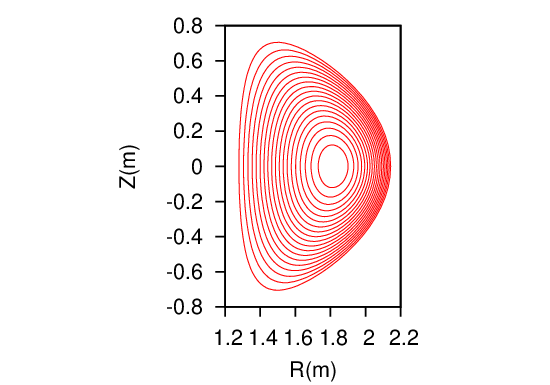
\includegraphics{/home/yj/project_new/fft/fig3/tmp2.eps}}
  \caption{\label{8-27-p1}The real (left) and imaginary (right) part of the
  discrete Fourier transformation as a function of the frequency. The point $n
  = - 128$ corresponds to frequency $- f_s / 2$ while the point $n = 128$
  corresponds to frequency $+ f_s / 2$, where $f_s = 1 / \Delta$ with $\Delta$
  is the sample interval in time domain. The time domain data is the same as
  used in Fig. \ref{3-25-e8}. Why is there a spike at zero frequency?}
\end{figure}

\

\

\subsection{Computing Fourier integrals using FFT (not finished, to be
deleted)}

Consider the calculation of the following integral:
\begin{equation}
  \label{8-26-1} I (\omega) = \int_a^b e^{i \omega t} h (t) d t.
\end{equation}
Divide the interval $[a, b]$ into $M$ uniform sub-intervals and define
\begin{equation}
  \Delta = \frac{b - a}{M}, t_j = a + \Delta j, h_j = h (t_j), j = 0, 1, 2,
  \ldots, M
\end{equation}
Then the integration in Eq. (\ref{8-26-1}) can be approximated as
\begin{equation}
  \label{8-26-e1} I (\omega) \approx \Delta \sum_{j = 0}^{M - 1} h_j \exp (i
  \omega t_j) .
\end{equation}
Define $\omega_m = 2 \pi m / (M \Delta)$ with integer $m$ and $- M / 2 < m < M
/ 2$. Consider the calculation of $I (\omega_m)$. Using Eq. (\ref{8-26-e1}),
we obtain
\begin{eqnarray}
  I (\omega_m) & = & \Delta \sum_{j = 0}^{M - 1} h_j \exp [i \omega_m (a +
  \Delta j)] \nonumber\\
  & = & \Delta e^{i \omega_m a} \sum_{j = 0}^{M - 1} h_j \exp (i \omega_m
  \Delta j) \nonumber\\
  & = & \Delta e^{i \omega_m a} \sum_{j = 0}^{M - 1} h_j \exp \left( i
  \frac{2 \pi m}{M} j \right) \nonumber\\
  & = & \Delta e^{i \omega_m a} H_m \\
  & = & \Delta e^{i \omega_m a} [\tmop{DFT} (h_0, h_1, h_2, \ldots, h_{M -
  1})]_m .  \label{8-26-e2}
\end{eqnarray}
Equation (\ref{8-26-e2}) indicates the value of the integration $I (\omega_m)$
can be obtained by calculating the discrete Fourier transformation of $h_j$.
However, as discussed in Ref. {\cite{press1992}}, equation (\ref{8-26-e2}) is
not recommended for practical use because the oscillatory nature of the
integral will make Eq. (\ref{8-26-e2}) become systematically inaccurate as
$\omega$ increases. Next, consider a new method, in which $h (t)$ is expanded
as
\begin{equation}
  \label{8-27-1} h (t) \approx \sum_{j = 0}^M h_j \psi \left( \frac{t -
  t_j}{\Delta} \right) + \sum_{j = \tmop{endpoints}} h_j \varphi_j \left(
  \frac{t - t_j}{\Delta} \right)
\end{equation}
Apply the integral operator$\int_a^b d t \exp (i \omega t)$ to both sides of
Eq. (\ref{8-27-1}), we obtain
\begin{equation}
  \int_a^b h (t) e^{i \omega t} d t \approx \sum_{j = 0}^M h_j \int_a^b \psi
  \left( \frac{t - t_j}{\Delta} \right) e^{i \omega t} d t + \sum_{j =
  \tmop{endpoints}} h_j \int_a^b \varphi_j \left( \frac{t - t_j}{\Delta}
  \right) e^{i \omega t} d t.
\end{equation}
Make the change of variables $s = (t - t_j) / \Delta$ in the first integral
and $s = (t - a) / \Delta$ in the second integral, the above equation is
written as
\begin{equation}
  \int_a^b h (t) e^{i \omega t} d t \approx \Delta \sum_{j = 0}^M h_j \int_a^b
  \psi (s) e^{i \omega (\Delta s + t_j)} d s + \Delta \sum_{j =
  \tmop{endpoints}} h_j \int_a^b \varphi_j (s - j) e^{i \omega (\Delta s + a)}
  d s
\end{equation}
Define $\theta = \omega \Delta$ and make use of $t_j = a + j \Delta$, the
above equation is written as
\begin{equation}
  \label{8-27-5} \int_a^b h (t) e^{i \omega t} d t \approx \Delta e^{i \omega
  a} \sum_{j = 0}^M h_j e^{i \theta j} \int_a^b \psi (s) e^{i \theta s} d s +
  \Delta e^{i \omega a} \sum_{j = \tmop{endpoints}} h_j \int_a^b \varphi_j (s
  - j) e^{i \theta s} d s
\end{equation}
Define
\begin{equation}
  W (\theta) = \int_a^b \psi (s) e^{i \theta s} d s
\end{equation}
\begin{equation}
  \alpha_j (\theta) = \int_a^b \varphi_j (s - j) e^{i \theta s} d s
\end{equation}
Then Eq. (\ref{8-27-5}) is written as
\begin{equation}
  \int_a^b h (t) e^{i \omega t} d t \approx \Delta e^{i \omega a} \left[ W
  (\theta) \sum_{j = 0}^M h_j e^{i \theta j} + \sum_{j = \tmop{endpoints}} h_j
  \alpha_j (\theta) \right] .
\end{equation}


\

\

\

\

\

\begin{figure}[h]
  \includegraphics{/home/yj/project_new/fft/fig2b/MyFigure.eps}
  \caption{Older version of Fig. \ref{4-16-1}, created by Metapost, the new
  version is created by the vector graphic editor in TeXmacs.}
\end{figure}

\

\begin{thebibliography}{1}
  \bibitem[1]{snieder1994}\tmtextit{A Guided Tour of Mathematical Physics}.
  {\newblock}Samizdat Press, 1994.
  
  \bibitem[2]{press1992}W.~H. Press, S.~A. Teukolsky, W.~T. Vetterling, and
  B.~P. Flannery. {\newblock}\tmtextit{Numerical Recipes in Fortran 77}.
  {\newblock}Cambridge University Press, Cambridge, UK, 1992.
\end{thebibliography}

\

\

\end{document}
